% Module B - Prototype Functional Verification (test plan, procedures and test report)
% Compiles with XeLaTeX (Overleaf: Menu -> Compiler -> XeLaTeX) or `tectonic main.tex`.
\documentclass[10pt,a4paper]{article}

\usepackage{fontspec}
\IfFontExistsTF{Times New Roman}{\setmainfont{Times New Roman}}{\setmainfont{TeX Gyre Termes}}
\usepackage[a4paper,margin=2cm,top=2cm,bottom=2.2cm]{geometry}
\usepackage{graphicx}
\usepackage{array,tabularx,longtable,multirow}
\usepackage[table]{xcolor}
\usepackage{amsmath}
\usepackage{pifont}
\usepackage{enumitem}
\usepackage{float}
\usepackage{caption}
\usepackage{subcaption}
\usepackage{titlesec}
\usepackage{tikz}
\usetikzlibrary{positioning,arrows.meta,shapes.geometric,calc}
\usepackage[hidelinks]{hyperref}
\hypersetup{pdftitle={Autonomous UAV System for Forest Fire Monitoring - Module B Test Report}}

\setlength{\parindent}{0pt}
\setlength{\parskip}{4pt}
\renewcommand{\arraystretch}{1.18}
\captionsetup{font=small,labelfont=bf,labelsep=colon}
\captionsetup[sub]{font=small}
\setlist{itemsep=1pt,topsep=3pt}
\titleformat{\section}{\Large\bfseries}{\thesection}{0.6em}{}
\titleformat{\subsection}{\large\bfseries}{\thesubsection}{0.6em}{}
\titlespacing*{\section}{0pt}{10pt}{6pt}
\titlespacing*{\subsection}{0pt}{8pt}{4pt}
\newcolumntype{L}[1]{>{\raggedright\arraybackslash}p{#1}}
\newcolumntype{Y}{>{\raggedright\arraybackslash}X}

\definecolor{passgreen}{HTML}{1E7B34}
\definecolor{warnamber}{HTML}{A65F00}
\definecolor{failred}{HTML}{B3261E}
\definecolor{headgray}{HTML}{F2F2F2}
\newcommand{\PASS}{\textcolor{passgreen}{\textbf{\ding{51}\,PASS}}}
\newcommand{\FAIL}{\textcolor{failred}{\textbf{\ding{55}\,FAIL}}}
\newcommand{\PART}{\textcolor{warnamber}{\textbf{PASS*}}}
\newcommand{\EXP}{\textcolor{warnamber}{\textbf{EXPERT CHECK}}}
\newcommand{\head}[1]{\textbf{#1}}
\newcommand{\file}[1]{\texttt{\small #1}}

\tikzset{box/.style={draw,rounded corners=3pt,align=center,font=\small,minimum height=9mm,inner sep=4pt},
         arr/.style={-{Stealth[length=2.2mm]},thick}}

\begin{document}

% ------------------------------------------------------------------ cover
\begin{titlepage}
\centering
{\large\bfseries BRICS HIGHSKILLS 2026\par}
\vspace{2pt}
{\bfseries AERIAL ROBOTICS COMPETITION\par}
\vspace{2pt}
{Prototype Functional Verification\par}
\vspace{10pt}
\rule{\textwidth}{0.6pt}
\vspace{18pt}

\raggedright
{\large\bfseries CASE 1\par}
\vspace{8pt}
{\fontsize{22}{26}\selectfont\bfseries AUTONOMOUS UAV SYSTEM\\FOR FOREST FIRE MONITORING\par}
\vspace{8pt}
{\large Test plan, procedures, test report\\and corrective actions\par}
\vspace{18pt}

\centering
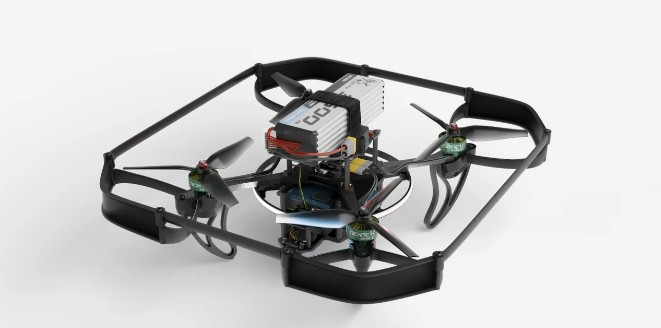
\includegraphics[width=0.62\textwidth]{figures/drone_cover.png}\par
\vspace{4pt}
{\small\textbf{Figure 1:} SKYRIS TECHNIC 6S --- prototype under verification\par}
\vspace{22pt}

{\Large\bfseries TEAM ENTITY\par}
{\Large\bfseries Workstation Number: 5\par}
\vspace{16pt}

\begin{tabularx}{\textwidth}{|L{3.2cm}|Y|}
\hline
\head{Competition} & BRICS HIGHSKILLS 2026 --- Aerial Robotics \\ \hline
\head{Case Study} & Autonomous UAV System for Forest Fire Monitoring \\ \hline
\multirow{2}{*}{\head{Team Members}} & Kamalesh Vadivelu Syamala \\
 & Bejin Paul Josephin Paul Benjamin \\ \hline
\head{Document} & Module B --- Prototype Functional Verification \\ \hline
\head{Test period} & 9--11 November 2026, competition flight area, Yekaterinburg \\ \hline
\head{Revision} & November 2026 \\ \hline
\end{tabularx}
\end{titlepage}
\setcounter{figure}{1}

% ------------------------------------------------------------------ executive summary
\section*{Executive Summary}
\vspace{-6pt}\rule{\textwidth}{0.4pt}

This report documents the functional verification of the autonomous forest-fire monitoring UAV described in the Module~A
technical report. It contains the test plan and procedures defined before testing, the results of software, bench, flight
and end-to-end tests, the defects found during testing and the corrective actions taken.

All results are taken from the run folders that the drone writes automatically for every mission
(\file{log.txt}, \file{path.csv}, \file{events.csv}, \file{perf.csv}, \file{objects.json}, \file{snapshots/}) and from the
ground dashboard that reads them. The charts in this report are generated from those files by a script in the project
repository (\file{make\_figures.py}), so every figure can be reproduced from the raw logs.

\textbf{Test campaign:} 61 mission starts were logged on 10--11 November 2026. 15 of them were complete autonomous
survey missions (take-off, full lawnmower route, detection, return, landing, report) without manual piloting. The
remaining attempts were stopped on the ground or before the survey (arming, OFFBOARD mode, operator stop) and were
recovered by restarting, as permitted by the test procedure.

\subsection*{Verification summary --- seven mandatory characteristics}

\begin{tabularx}{\textwidth}{|L{0.7cm}|L{4.0cm}|L{2.7cm}|Y|L{1.9cm}|}
\hline
\rowcolor{headgray}\head{ID} & \head{Characteristic} & \head{Threshold} & \head{Measured result} & \head{Verdict} \\ \hline
C1 & Autonomous flight along the predefined route & 100\,\% of waypoints, each $\le$ 0.25\,m & 15/15 flights, 100\,\% of waypoints; worst 0.09\,m & \PASS \\ \hline
C2 & NN flame detection in thermal images & mAP@0.5 $\ge$ 0.85 & 0.993 (fire / campfire class), 0.905 all classes, held-out flight & \PASS \\ \hline
C3 & Additional object (trees) & every tree, correct class & 3--5 trees mapped in each of the 4 tree flights & \PASS \\ \hline
C4 & Onboard NPU processing rate & $\ge$ 10\,FPS for $>$ 90\,\% of airborne time & RGB 100\,\%; thermal 94.8\,\% / 93.6\,\% in the final flights & \PASS \\ \hline
C5 & Object coordinate accuracy & $\le$ 0.5\,m & repeat spread $\le$ 0.28\,m (4 flights); $\le$ 0.05\,m fire error in simulation & \PART \\ \hline
C6 & Live map display (type + time) & $\le$ 2\,s & displayed with type, X/Y and time; 0.7\,s refresh & \PART \\ \hline
C7 & Autonomous return on command & reaction $\le$ 2\,s, landing $\le$ 0.5\,m & reaction $<$ 1\,s (sim); return error $\le$ 0.18\,m (15 flights) & \PART \\ \hline
\end{tabularx}

{\small \PART\ = the threshold is met by the recorded evidence, and the final measurement is made by the expert
during the scored attempt with the method in Section~2 (tape measurement for C5, screen recording for C6, operator
RETURN press in flight for C7).}

\textbf{Key outcome:} testing found ten defects. All of them were corrected: five were re-verified in flight and the rest on the bench or by unit tests. The
most important was a thermal-camera stream dropout that caused C4 to fail in seven flights; after the fix, the final
two flights passed C4 on both streams.

% ------------------------------------------------------------------ 1
\section{Test Scope, Environment and Approach}

\subsection{Objective}
The objective of Module~B is to verify that the prototype meets the requirements of Case~1 (University 2035) with
measurable thresholds, to identify defects, to correct them and to re-test the corrected system.

\subsection{System under test}
SKYRIS TECHNIC 6S (PX4 v1.17.0) with an Orange Pi 5 Pro (RK3588S NPU), downward TR256i thermal camera (256 $\times$ 192,
$^\circ$C per pixel) and RGB camera (640 $\times$ 480), ArUco + optical-flow + rangefinder navigation, thermal YOLO11n
(\texttt{fire}, \texttt{flame}, \texttt{tree\_fire}) and RGB YOLO11n (\texttt{fire}, \texttt{tree}) on the NPU, and the BRICS
Dashboard ground station --- as specified in the Module~A technical report.

\subsection{Test environment}
\begin{itemize}
  \item Competition flight area: netted arena with a 3.5\,m ceiling and the organiser's ArUco floor map.
  \item Simulated campfire: a heated disc (52--88\,$^\circ$C measured from flight height) and red flame lamps.
  \item Additional objects: artificial trees, each with a heat band of about 40--55\,$^\circ$C (``tree fire'').
  \item Survey area $x \in [-2.5, 2.5]$, $y \in [-1, 1]$\,m; geofence $x \in [-3.3, 3.3]$, $y \in [-1.75, 1.75]$\,m;
        home pad at the map origin.
  \item Each flight-area visit is limited to 10 minutes; one survey mission takes 64--152\,s.
\end{itemize}

\subsection{Test levels and evidence chain}
Testing was performed at four levels: (1) software unit and simulation tests on the laptop, (2) bench tests
with the drone on the ground, (3) single-function flight tests (hover, ArUco roam), and (4) full end-to-end missions.

\begin{figure}[!htb]
\centering
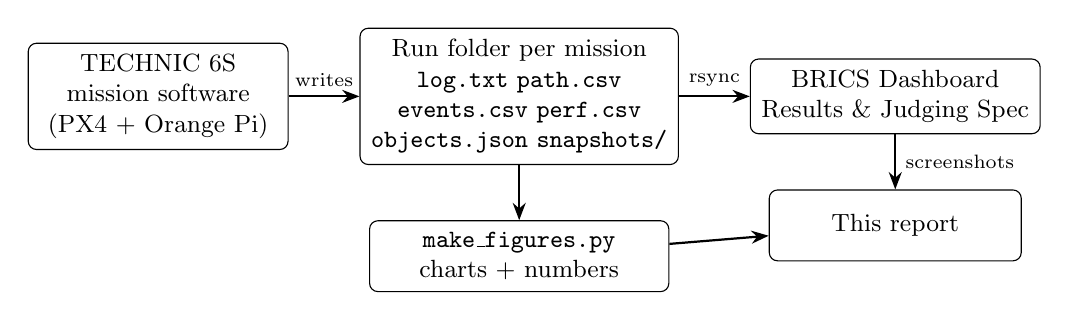
\begin{tikzpicture}[node distance=7mm and 9mm]
\node[box,minimum width=33mm] (drone) {TECHNIC 6S\\mission software\\(PX4 + Orange Pi)};
\node[box,right=of drone,minimum width=38mm] (run) {Run folder per mission\\\file{log.txt} \file{path.csv}\\\file{events.csv} \file{perf.csv}\\\file{objects.json} \file{snapshots/}};
\node[box,right=of run,minimum width=32mm] (dash) {BRICS Dashboard\\Results \& Judging Spec};
\node[box,below=of run,minimum width=38mm] (fig) {\file{make\_figures.py}\\charts + numbers};
\node[box,below=of dash,minimum width=32mm] (rep) {This report};
\draw[arr] (drone) -- node[above,font=\scriptsize]{writes} (run);
\draw[arr] (run) -- node[above,font=\scriptsize]{rsync} (dash);
\draw[arr] (run) -- (fig);
\draw[arr] (fig) -- (rep);
\draw[arr] (dash) -- node[right,font=\scriptsize]{screenshots} (rep);
\end{tikzpicture}
\caption{Evidence chain: every number in this report can be traced back to a file written by the drone.}
\end{figure}

% ------------------------------------------------------------------ 2
\section{Test Plan and Procedures}

The test programme below was fixed before the flight tests and is stored in the project repository
(\file{deliverables/case1\_forest\_fire/04\_Test\_Programme.md}) and in the dashboard ``Judging Spec'' section.
Thresholds and methods were not changed after testing started.

\subsection{Seven mandatory verifiable characteristics}

\begin{longtable}{|L{0.6cm}|L{3.1cm}|L{1.7cm}|L{2.3cm}|L{5.6cm}|L{1.2cm}|}
\hline
\rowcolor{headgray}\head{ID} & \head{Characteristic} & \head{Unit} & \head{Threshold} & \head{Measurement method} & \head{Attempts} \\ \hline
\endfirsthead
\hline
\rowcolor{headgray}\head{ID} & \head{Characteristic} & \head{Unit} & \head{Threshold} & \head{Measurement method} & \head{Attempts} \\ \hline
\endhead
C1 & Autonomous flight along the predefined route & \% of planned waypoints & 100\,\%, each within 0.25\,m, no RC input & Planned lawnmower waypoints (\file{log.txt} \texttt{[plan]}) compared with the flown path (\file{path.csv}); RC sticks untouched on video. & 3 \\ \hline
C2 & NN detection of the simulated flame in thermal images & mAP@0.5 & $\ge$ 0.85 & Thermal frames of the scored flight, ground-truth boxes checked by the expert, Ultralytics \texttt{val} with the flight model. & 3 \\ \hline
C3 & Detection of an additional object (trees) & detected / present & every tree in the area, correct class & Confirmed \texttt{tree} entries in \file{objects.json} compared with the trees placed in the field. & 3 \\ \hline
C4 & Onboard NPU/GPU processing rate & FPS per 1-s interval & $\ge$ 10\,FPS in $>$ 90\,\% of airborne 1-s intervals & Every perception cycle is time-stamped in \file{perf.csv}; \file{fps\_summary.json} gives the share of intervals $\ge$ 10\,FPS. & 3 \\ \hline
C5 & Accuracy of object coordinates & m (horizontal) & $\le$ 0.5\,m for every confirmed object & Expert tape measurement from the marker-map origin, entered in the dashboard and compared with the reported X/Y. & 3 \\ \hline
C6 & Real-time map display with type and timestamp & s after confirmation & $\le$ 2\,s & Screen recording of the dashboard compared with the confirmation time in \file{events.csv}. & 3 \\ \hline
C7 & Autonomous return on operator command & s (reaction), m (landing) & reaction $\le$ 2\,s; landing $\le$ 0.5\,m from home & \file{log.txt}: \texttt{operator pressed RETURN} $\rightarrow$ \texttt{[phase] RETURN}; landing point vs home pad. & 3 \\ \hline
\end{longtable}

\subsection{Detailed test procedures}

Each procedure lists the initial conditions, the sequence of actions and the pass criterion. Common initial conditions
for all flight tests: Module~A pre-test checklist complete, battery $\ge$ 3.8\,V/cell, drone on the home pad,
drone clock synchronised with the laptop, video recording started.

\begin{longtable}{|L{0.6cm}|L{3.6cm}|L{7.1cm}|L{3.7cm}|}
\hline
\rowcolor{headgray}\head{ID} & \head{Initial conditions} & \head{Sequence of actions} & \head{Pass criterion} \\ \hline
\endfirsthead
\hline
\rowcolor{headgray}\head{ID} & \head{Initial conditions} & \head{Sequence of actions} & \head{Pass criterion} \\ \hline
\endhead
C1 & Survey area and altitude set in Mission settings; geofence active & 1.~Press \textbf{Run mission}. 2.~Drone takes off, flies the lawnmower lines, returns and lands. 3.~Compute the distance from each planned waypoint to the flown path. & All waypoints reached within 0.25\,m; no RC input \\ \hline
C2 & Campfire placed by the expert at an unknown position & 1.~Fly the scored mission; thermal frames are saved every 1\,s. 2.~Team labels the frames; expert checks the labels. 3.~Run \texttt{val} with the deployed model. & mAP@0.5 $\ge$ 0.85 for the campfire class \\ \hline
C3 & Trees placed in the area & 1.~Fly the mission. 2.~Count confirmed \texttt{tree} objects and compare with the trees present. & Every tree confirmed once, class \texttt{tree} \\ \hline
C4 & Both cameras streaming; dashboard shows live FPS & 1.~Fly the mission. 2.~Read \file{fps\_summary.json} (airborne span). & $>$ 90\,\% of airborne 1-s intervals $\ge$ 10\,FPS \\ \hline
C5 & Same flight as C2/C3 & 1.~After landing the expert measures each target's X, Y with a tape from the map origin. 2.~Values are entered in the dashboard (Judging Spec $\rightarrow$ C5). 3.~Dashboard computes the error per object. & Every object $\le$ 0.5\,m \\ \hline
C6 & Screen recording of the dashboard running & 1.~Fly the mission. 2.~For each confirmation in \file{events.csv}, find the first video frame that shows the object on the map. & Delay $\le$ 2\,s; type and time shown \\ \hline
C7 & Mission running, drone on the survey & 1.~At a moment chosen by the expert, press \textbf{Return Home}. 2.~Drone flies home and lands. 3.~Compare log times and landing point. & Reaction $\le$ 2\,s; landing $\le$ 0.5\,m \\ \hline
\end{longtable}

\subsection{Three functional modules}
\begin{tabularx}{\textwidth}{|L{2.6cm}|L{4.5cm}|L{4.0cm}|Y|}
\hline
\rowcolor{headgray}\head{Module} & \head{Contents} & \head{Separately verifiable function} & \head{Pass criterion} \\ \hline
M1 --- Flight and navigation & PX4, SKYRIS \texttt{simple\_offboard}, ArUco map + optical flow + rangefinder, mission planner, safety layer & Autonomous take-off to 1.5\,m, 5\,s position hold, landing (\file{tools/hover\_test.py}) & Height 1.5 $\pm$ 0.15\,m; drift $\le$ 0.2\,m; lands and disarms without RC \\ \hline
M2 --- Thermal perception & TR256i $^\circ$C stream, thermal YOLO + RGB YOLO on the NPU, temperature confirmation, tracker & Campfire under the drone is confirmed as \texttt{fire} & Confirmed $\le$ 3\,s, confidence $\ge$ 0.5, $\ge$ 10\,FPS \\ \hline
M3 --- Ground station and logging & Operator UI, BRICS Dashboard, \file{events.csv}, report & A detection appears on the map; commands are acknowledged & Type, X/Y and time on the map; row in \file{events.csv}; command logged $\le$ 1\,s \\ \hline
\end{tabularx}

\subsection{End-to-end scenario}
\textbf{Initial conditions:} drone on the home pad; campfire and trees placed by the expert; mission configuration loaded;
dashboard connected; video recording running.

\textbf{Sequence:} (1) operator presses \textbf{Run mission}; (2) automatic pre-flight checks (battery, position on the
marker map, on ground); (3) take-off and climb to survey altitude; (4) lawnmower survey; (5) on each confirmed ignition
source: red LED alarm, position hold, RGB + thermal snapshots, resume; (6) trees mapped without stopping;
(7) return home (end of route, or operator command); (8) landing and disarm; (9) report generated.

\textbf{Pass criteria:} campfire detected at least once; C1--C7 thresholds met; every detection logged with time, X/Y,
class and confidence; no manual piloting; total time $\le$ 9\,min.

\textbf{Attempts:} 3 within the flight-area slots. \textbf{Permitted recovery:} battery swap; restart of the mission from
the dashboard; placing the drone back on the pad; automatic safety landing followed by a restart.
\textbf{Prohibited during the formal scenario:} any change to source code, configuration files or hardware.

\subsection{Additional functions (outside the mandatory specification)}
\begin{tabularx}{\textwidth}{|L{0.8cm}|L{4.2cm}|Y|L{3.0cm}|L{2.1cm}|}
\hline
\rowcolor{headgray}\head{No.} & \head{Function} & \head{Verification scenario} & \head{Pass criterion} & \head{New component} \\ \hline
AF1 & Inspection hold on every confirmed ignition source & Normal mission with the campfire in the area & Hold + RGB/thermal snapshot pair + LED alarm logged & Yes (mission logic) \\ \hline
AF2 & Automatic safety layer (geofence, altitude, battery, marker loss, time limit) & Unit tests with simulated faults; mission with the configured fence & Automatic landing with the reason in \file{log.txt} & Yes (safety layer) \\ \hline
AF3 & In-flight camera self-calibration from repeated views of the same object & Normal mission; compare the spread of views before/after & Views agree better after calibration; logged & Yes (\file{selfcal}) \\ \hline
\end{tabularx}

% ------------------------------------------------------------------ 3
\section{Software Testing}

\subsection{Automated test suites}
Software tests were run on the laptop against the same mission code that runs on the drone, using a simulated drone and
simulated cameras. Results of the run on 12 November 2026:

\begin{tabularx}{\textwidth}{|L{5.2cm}|Y|L{2.1cm}|}
\hline
\rowcolor{headgray}\head{Test suite} & \head{What it checks} & \head{Result} \\ \hline
Flight-safety unit tests (\file{tests/test\_flight\_safety.py}) & Geofence, altitude limit, low battery, marker loss, time limit, stop = land (never disarm in flight), return-on-flame mission, self-calibration range, tree and heat-band mapping & 35/35 \PASS \\ \hline
Quick system suite (\file{tests/run\_all\_tests.py --quick}) & Python compile, thermal decode and camera discovery on any USB port, mock missions (includes the stress test below) & 8 of 9 pass \\ \hline
Venue rehearsal stress test (\file{tests/sim\_case1\_venue.py}) & Full mission with deliberately wrong camera models (lens $\pm$30--40\,\%, cameras upside down, position jitter) & 3/8 scenarios \\ \hline
\end{tabularx}

The stress test passes all scenarios with a correct camera model (perfect cameras, and 8\,cm / 3$^\circ$ position jitter).
It fails only when both cameras are deliberately mounted upside down \emph{and} have wrong lenses: in those cases the
mission still completes, but some tree positions are wrong by more than 0.5\,m before self-calibration converges. On the
real drone the camera mounting is fixed and checked, so these scenarios are a robustness margin, not a test of the flight
configuration.

Position errors against simulated ground truth (correct cameras, with and without position jitter):

\begin{tabularx}{\textwidth}{|L{3.4cm}|Y|Y|Y|Y|}
\hline
\rowcolor{headgray}\head{Scenario} & \head{Fire (campfire)} & \head{Flame lamp} & \head{Trees} & \head{Tree heat band} \\ \hline
Perfect cameras & 0.00\,m & 0.00\,m & 0.02 / 0.08\,m & 0.41 / 0.24\,m \\ \hline
Jitter 8\,cm, 3$^\circ$ & 0.05\,m & 0.03\,m & 0.05 / 0.13\,m & 0.43 / 0.15\,m \\ \hline
\end{tabularx}

\subsection{Thermal neural-network validation (C2)}
The deployed thermal model was validated with Ultralytics \texttt{val} at 256\,px on a held-out set: 328 thermal frames
from flights that were \emph{not} used for training (247 frames without targets, to measure false alarms).

\begin{tabularx}{\textwidth}{|L{3.4cm}|Y|Y|Y|Y|Y|}
\hline
\rowcolor{headgray}\head{Class} & \head{Instances} & \head{Precision} & \head{Recall} & \head{mAP@0.5} & \head{mAP@0.5:0.95} \\ \hline
\textbf{fire (campfire)} & 47 & 0.933 & 0.979 & \textbf{0.993} & 0.841 \\ \hline
flame (lamp) & 34 & 0.936 & 0.861 & 0.979 & 0.699 \\ \hline
tree\_fire (heat band) & 4 & 0.636 & 1.000 & 0.745 & 0.629 \\ \hline
\textbf{all classes} & 85 & 0.835 & 0.947 & \textbf{0.905} & 0.723 \\ \hline
\end{tabularx}

\begin{figure}[!htb]
\centering
\begin{subfigure}{0.48\textwidth}\centering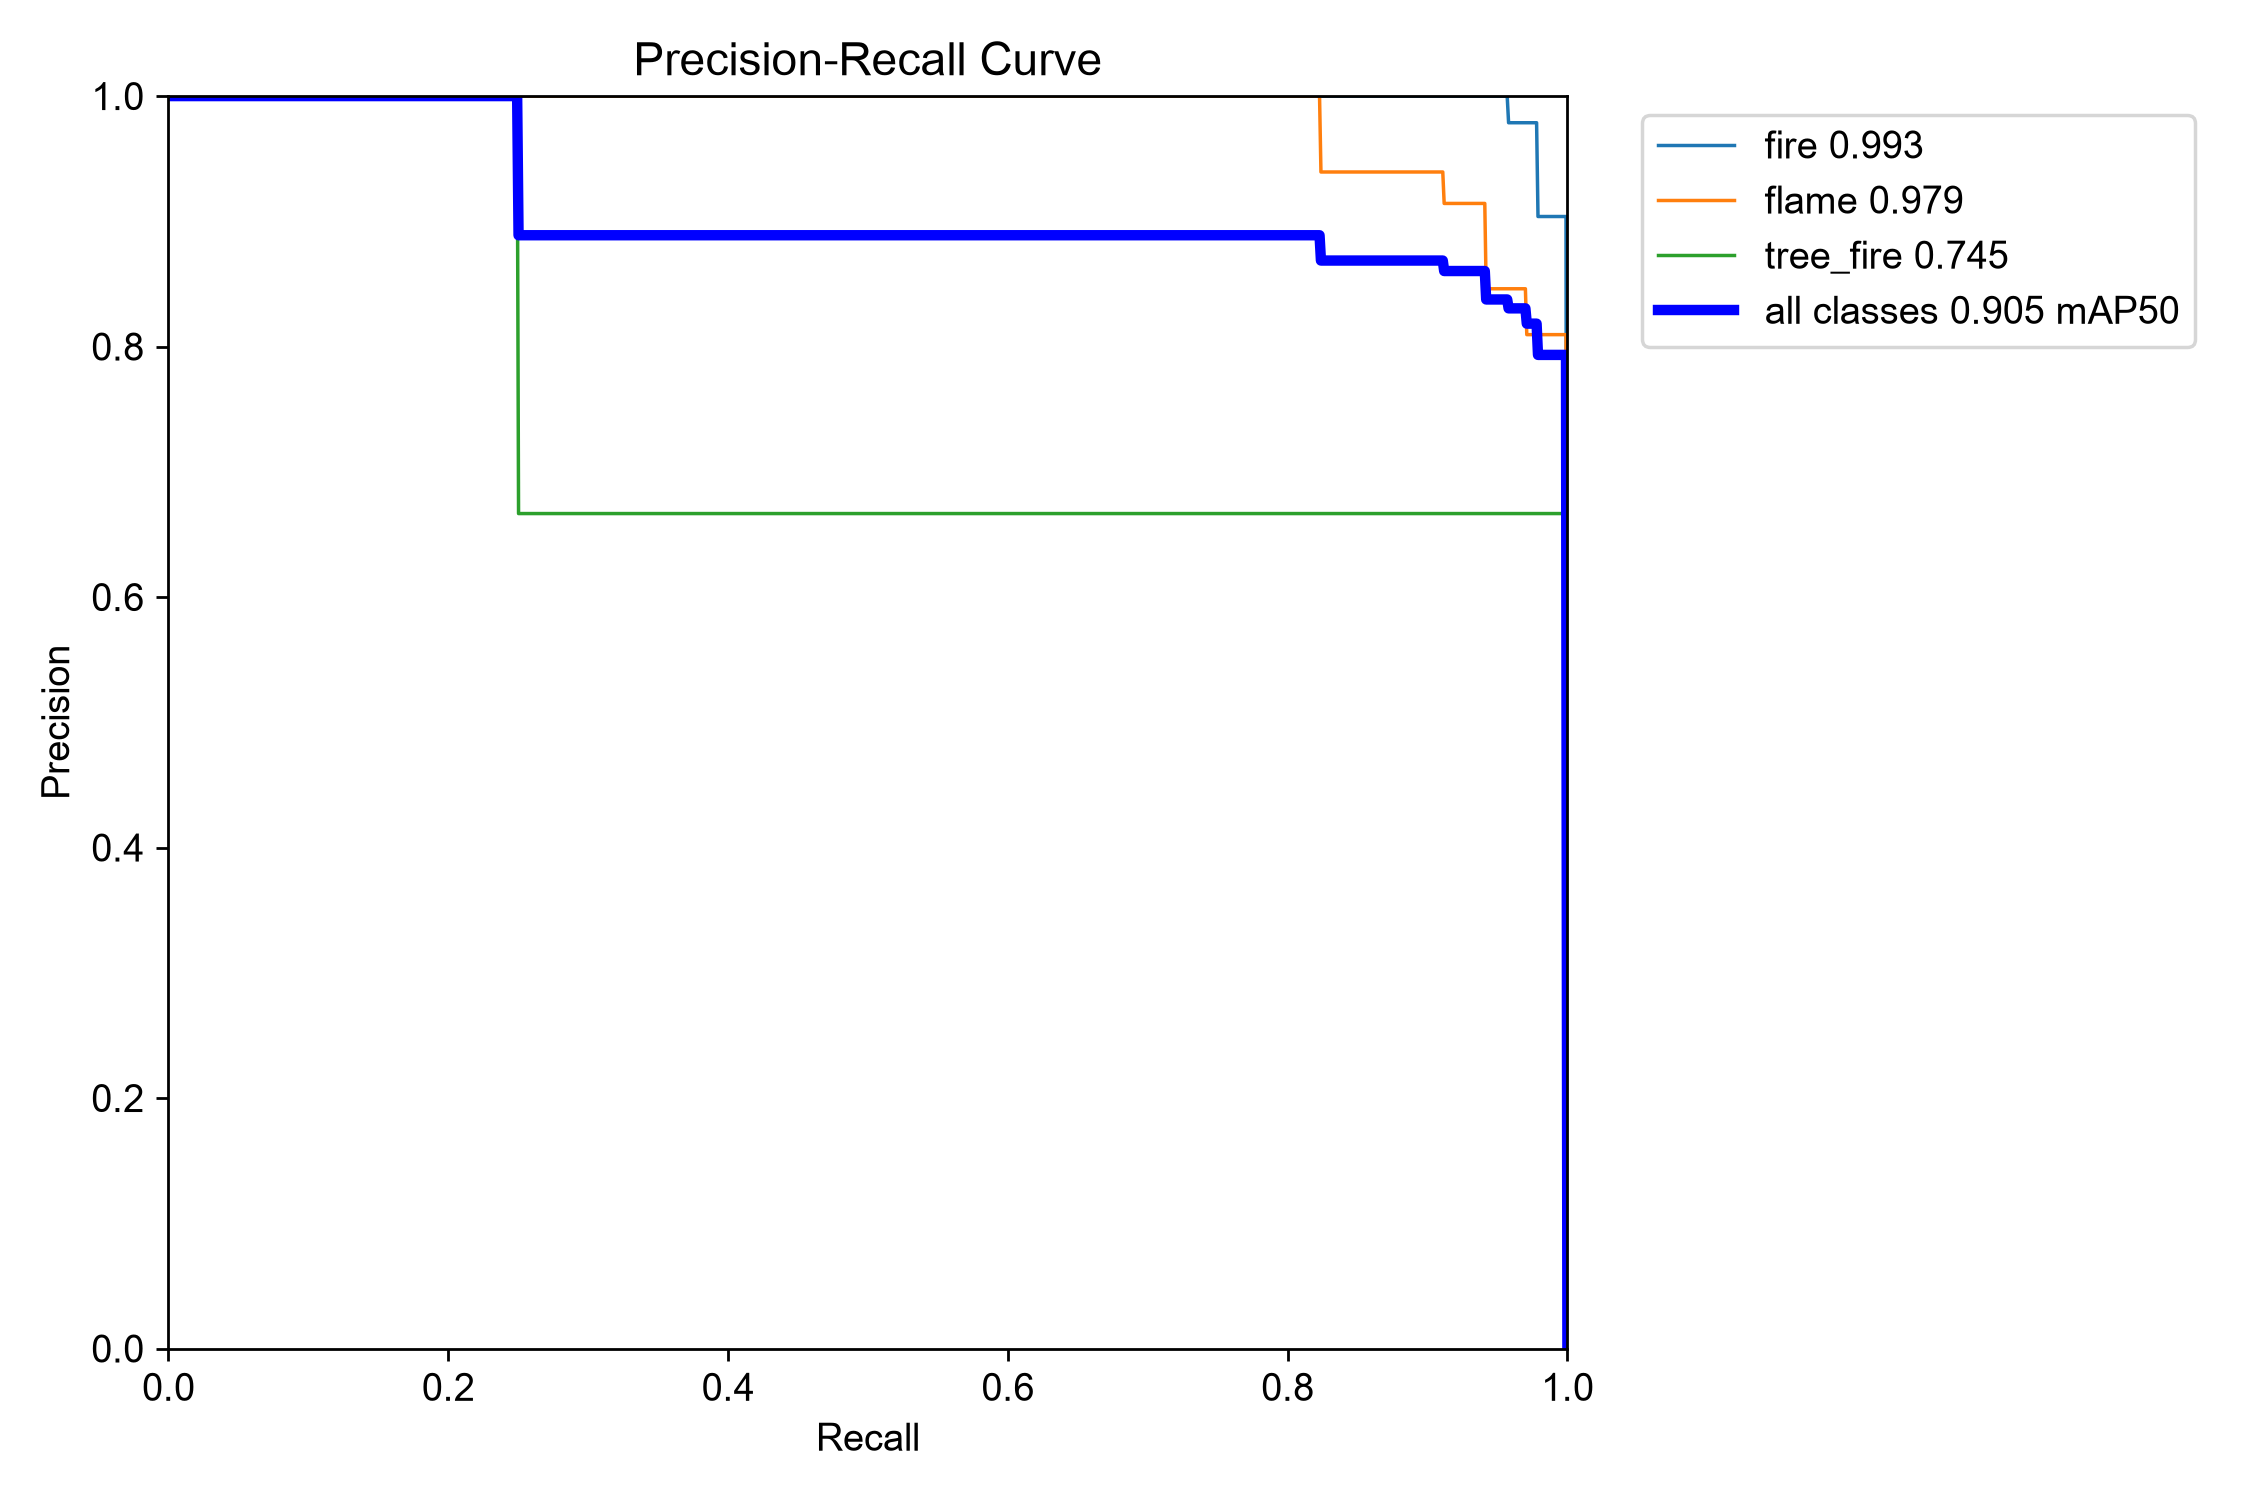
\includegraphics[width=\linewidth]{figures/thermal_pr.png}\caption{Precision--recall curve}\end{subfigure}\hfill
\begin{subfigure}{0.48\textwidth}\centering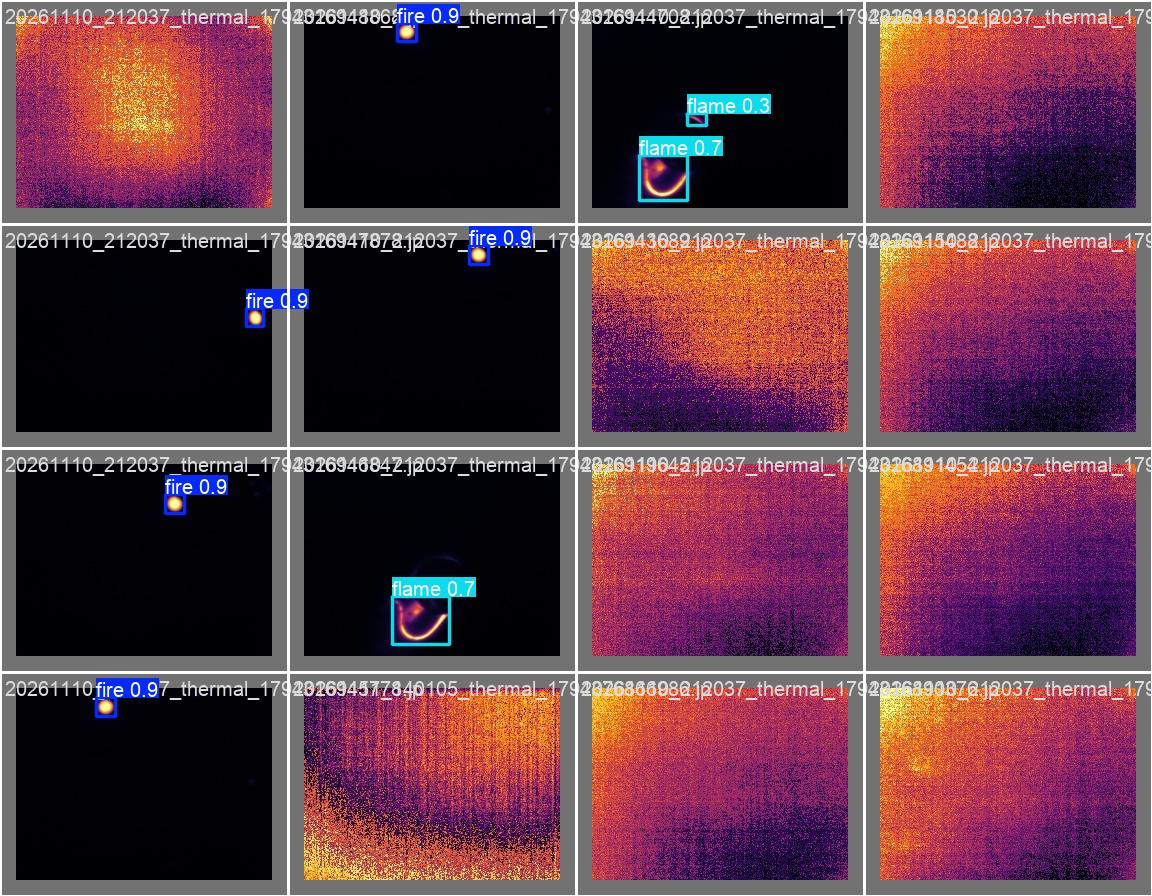
\includegraphics[width=\linewidth]{figures/thermal_valpred.jpg}\caption{Predictions on held-out frames (boxes: class, confidence)}\end{subfigure}
\caption{Thermal NN validation of the deployed model (\file{models/thermal\_fire}) on the 328 held-out flight frames.}
\end{figure}

The RGB detector (\texttt{fire} + \texttt{tree}, 856 training images) reaches mAP@0.5 = 0.995 for flame and 0.739 for
tree on its validation set (\file{models/fire/metrics.md}).


% ------------------------------------------------------------------ 4
\section{Flight Test Campaign}

\subsection{Single-function flight tests (module M1)}
\begin{tabularx}{\textwidth}{|L{3.2cm}|L{2.0cm}|Y|Y|L{2.6cm}|L{1.6cm}|}
\hline
\rowcolor{headgray}\head{Log} & \head{Target} & \head{Hold height (mean, min--max)} & \head{Horizontal drift in hold} & \head{End state} & \head{Verdict} \\ \hline
\file{hover\_20261109\_172036} & 1.5\,m, 5\,s & 1.42\,m (1.37--1.45) & 0.08\,m & landed, disarmed & \PASS \\ \hline
\file{hover\_20261110\_132531} & 1.5\,m, 5\,s & 1.37\,m (1.36--1.39) & 0.03\,m & landed, disarmed & \PASS \\ \hline
\file{hover\_20261110\_132838} & 10\,s hold & 1.90\,m (1.87--1.94) & 0.05\,m & landed, disarmed & --- \\ \hline
\end{tabularx}

ArUco roam and lawnmower tests (\file{roam\_*.csv}, 22 logs on 10--11 November) confirmed marker-based navigation over the
whole field before the full missions were flown.

\subsection{Full autonomous missions}
Table~\ref{tab:flights} lists every complete autonomous mission. Survey altitude was raised from 1.5\,m to 2.7--2.8\,m on
11 November to see the whole field and to keep the trees (1.5\,m tall) clear of the drone.

\begin{table}[H]
\centering
\small
\begin{tabular}{|l|c|c|c|c|c|c|c|l|}
\hline
\rowcolor{headgray}\head{Flight} & \head{Alt.} & \head{Time} & \head{Dist.} & \head{WP} & \head{Max WP err.} & \head{RGB $\ge$10} & \head{Th. $\ge$10} & \head{Confirmed objects} \\ \hline
10 Nov 18:53 & 1.5 & 139\,s & 32.2\,m & 8 & 0.09\,m & 93.5\,\% & 92.8\,\% & 3 fire \\ \hline
10 Nov 18:57 & 1.5 & 148\,s & 34.2\,m & 8 & 0.05\,m & 98.6\,\% & 98.0\,\% & 4 fire \\ \hline
10 Nov 21:11 & 1.5 & 105\,s & 28.4\,m & 8 & 0.03\,m & 100\,\% & 100\,\% & 1 flame \\ \hline
10 Nov 21:20 & 1.5 & 118\,s & 28.9\,m & 8 & 0.04\,m & 100\,\% & 99.1\,\% & 2 flame \\ \hline
11 Nov 14:01 & 1.5 & 152\,s & 40.1\,m & 8 & 0.03\,m & 100\,\% & \textcolor{failred}{56.6\,\%} & 1 fire, 1 flame \\ \hline
11 Nov 14:09 & 2.5 & 124\,s & 37.3\,m & 6 & 0.06\,m & 100\,\% & 95.9\,\% & 2 fire, 1 flame \\ \hline
11 Nov 17:08 & 2.7 & 70\,s & 23.1\,m & 6 & 0.04\,m & 100\,\% & \textcolor{failred}{4.3\,\%} & 2 flame \\ \hline
11 Nov 17:56 & 2.7 & 75\,s & 18.8\,m & 4 & 0.03\,m & 100\,\% & \textcolor{failred}{83.8\,\%} & 3 fire \\ \hline
11 Nov 17:59 & 2.7 & 64\,s & 18.0\,m & 4 & 0.03\,m & 100\,\% & \textcolor{failred}{79.7\,\%} & 3 fire \\ \hline
11 Nov 18:01 & 2.7 & 64\,s & 17.5\,m & 4 & 0.03\,m & 98.4\,\% & 90.5\,\% & 3 fire \\ \hline
11 Nov 18:16 & 2.7 & 68\,s & 18.1\,m & 4 & 0.03\,m & 100\,\% & \textcolor{failred}{1.5\,\%} & 2 flame \\ \hline
11 Nov 21:58 & 2.7 & 75\,s & 18.1\,m & 4 & 0.03\,m & 100\,\% & \textcolor{failred}{70.3\,\%} & 4 tree, 3 fire, 1 tree\_fire \\ \hline
11 Nov 21:59 & 2.7 & 76\,s & 17.7\,m & 4 & 0.04\,m & 100\,\% & \textcolor{failred}{72.0\,\%} & 3 tree, 3 fire, 2 tree\_fire \\ \hline
11 Nov 23:05 & 2.8 & 97\,s & 28.3\,m & 8 & 0.03\,m & 100\,\% & 94.8\,\% & 4 tree, 3 fire, 2 tree\_fire \\ \hline
11 Nov 23:07 & 2.8 & 78\,s & 17.5\,m & 4 & 0.04\,m & 100\,\% & 93.6\,\% & 5 tree, 3 fire, 2 tree\_fire \\ \hline
\end{tabular}
\caption{All 15 complete autonomous missions (run folders \file{case1\_fire\_2026111x\_hhmmss}). WP = planned waypoints;
``$\ge$10'' = share of airborne 1-s intervals at $\ge$ 10\,FPS. Red = below the C4 threshold.}
\label{tab:flights}
\end{table}

\subsection{Attempts that did not complete and recovery}
\begin{tabularx}{\textwidth}{|L{6.6cm}|L{1.2cm}|Y|}
\hline
\rowcolor{headgray}\head{Outcome logged in \file{summary.json}} & \head{Count} & \head{Recovery (permitted method)} \\ \hline
Stopped by the operator (Ctrl+C / Abort) before or after take-off & 10 & Restart from the dashboard \\ \hline
Take-off rejected: arming timed out / drone did not arm & 6 & Check PX4 pre-arm in QGC, restart \\ \hline
Navigate rejected: copter not in OFFBOARD mode & 4 & Safety landing, restart \\ \hline
Pre-flight check failed / telemetry service no response & 2 & Drone back on the pad, restart \\ \hline
Mission started and stopped on the ground (no summary written) & 23 & Restart \\ \hline
\end{tabularx}

No attempt ended in a crash or an uncontrolled landing. Every abort ended on the ground or with an automatic landing.

% ------------------------------------------------------------------ 5
\section{Results by Characteristic}

\subsection{C1 --- Autonomous flight along the predefined route \hfill \PASS}
For every complete mission, the planned lawnmower waypoints were regenerated with the planner used on the drone
(\file{common/geometry.py}, \texttt{lawnmower}) from the \texttt{[plan]} line in \file{log.txt}. The distance from each
waypoint to the flown path (\file{path.csv}) was then computed. All 15 missions reached 100\,\% of their waypoints. The
worst waypoint error in the campaign was 0.09\,m, against a threshold of 0.25\,m. No mission used RC input.

\begin{figure}[!htb]
\centering
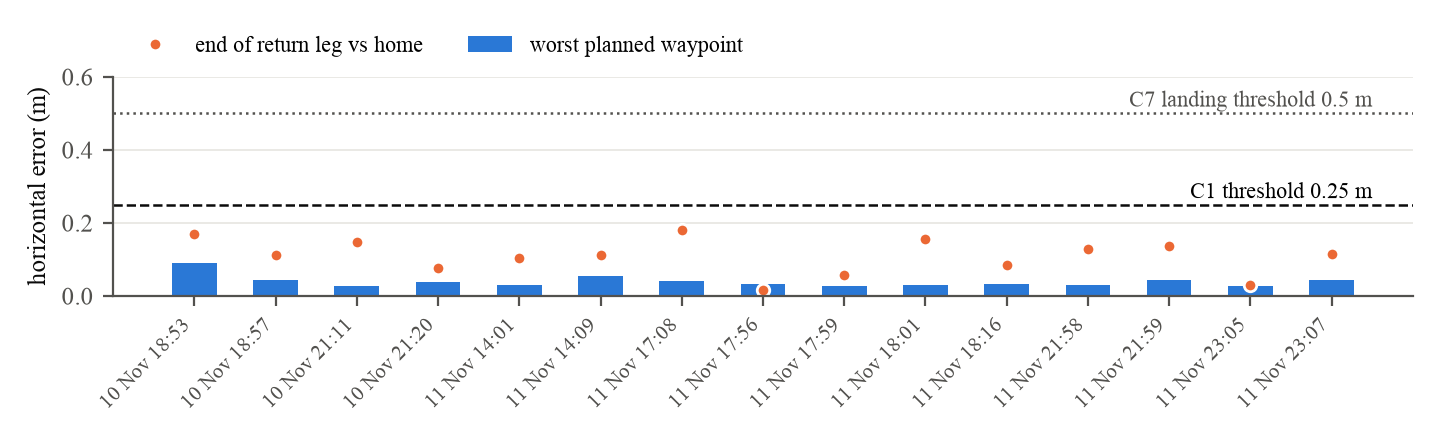
\includegraphics[width=\textwidth]{figures/chart_route.png}
\caption{Worst waypoint error per flight (C1) and distance between the end of the return leg and the home pad (C7).}
\end{figure}

\begin{figure}[!htb]
\centering
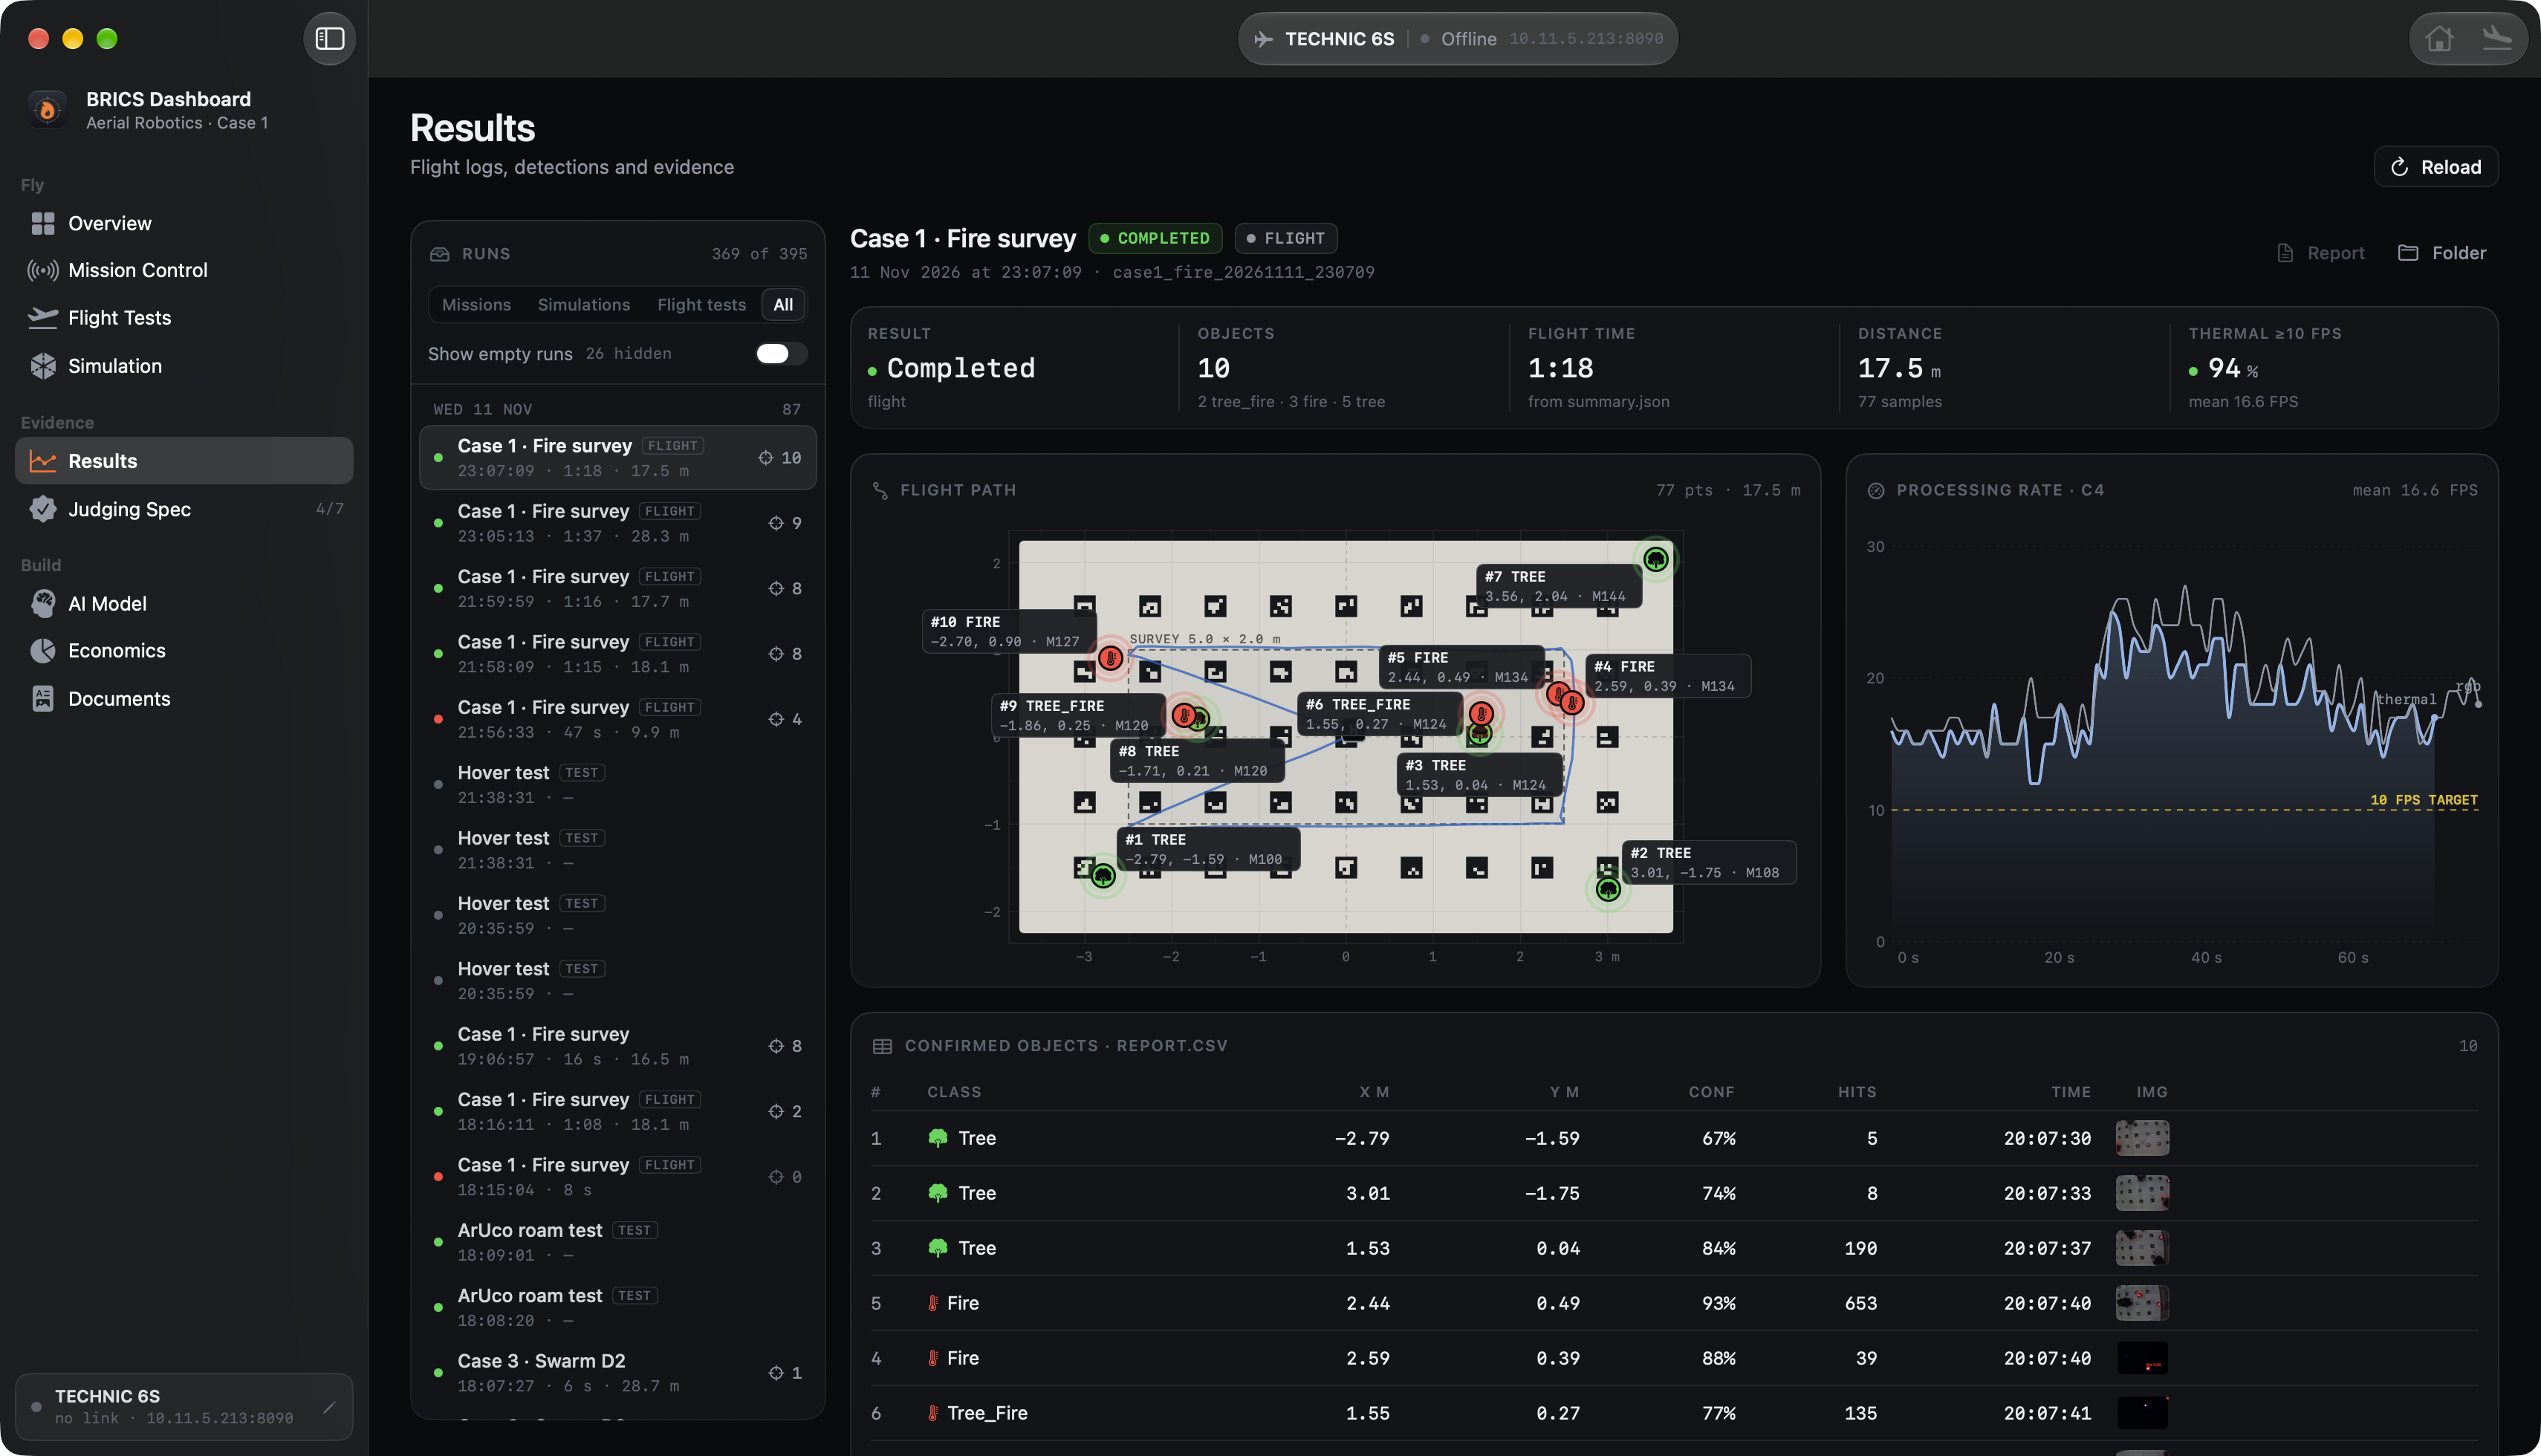
\includegraphics[width=\textwidth]{figures/dash_results.png}
\caption{Dashboard --- Results for the 11 Nov 23:07 flight: flown path and confirmed objects drawn on the real ArUco
floor map, processing rate (C4) and the confirmed-object table with class, X/Y, confidence, hits and time.}
\label{fig:results}
\end{figure}

\subsection{C2 --- Neural-network flame detection in thermal images \hfill \PASS}
On held-out thermal flight frames the deployed thermal NN reaches mAP@0.5 = \textbf{0.993} for the campfire class
(\texttt{fire}) and 0.905 over all classes (Section~3.2), above the 0.85 threshold. Detection is NN-only. Temperature is
used only to confirm NN boxes (fire $\ge$ 60\,$^\circ$C, flame $\ge$ 50\,$^\circ$C). In flight, a simulated flame (campfire or flame lamp) was confirmed in every one of the 15 complete missions. In the final
four flights the thermal NN confirmed each campfire at confidence 0.88--0.93 and 62--76\,$^\circ$C.
For the scored attempt, the same \texttt{val} procedure is run on that flight's frames with expert-checked labels.

\subsection{C3 --- Detection of an additional object (trees) \hfill \PASS}
The additional object selected by the team is the tree. Trees were placed in the arena from the evening of 11 November.
In all four flights after the trees were placed, the RGB NN confirmed and mapped 3--5 trees, each with an RGB and thermal
snapshot and no inspection stop. The three trees inside the survey area were found in every flight; the fourth, at the
fence edge, was found in 3 of 4 flights (Figure~\ref{fig:repeat}).
Trees were never reported as fire, and their heat bands were reported separately as \texttt{tree\_fire}.

\subsection{C4 --- Onboard NPU processing rate \hfill \PASS}
The RGB stream met the threshold in all 15 flights (93.5--100\,\% of airborne seconds at $\ge$ 10\,FPS). NPU inference is
not the bottleneck: the median detector call in \file{perf.csv} is 22.5--23.4\,ms in the final flights (capacity
$\approx$ 43\,FPS). The thermal stream failed C4 in seven flights. The logs show that thermal frames were missing at the
source while the RGB stream and the detector kept running, so the camera driver was the cause (defect D2,
Section~7). After the corrective action, the final two flights passed on both streams: thermal 94.8\,\% and 93.6\,\%
(mean 16.8 and 16.6\,FPS), RGB 100\,\%.

\begin{figure}[!htb]
\centering
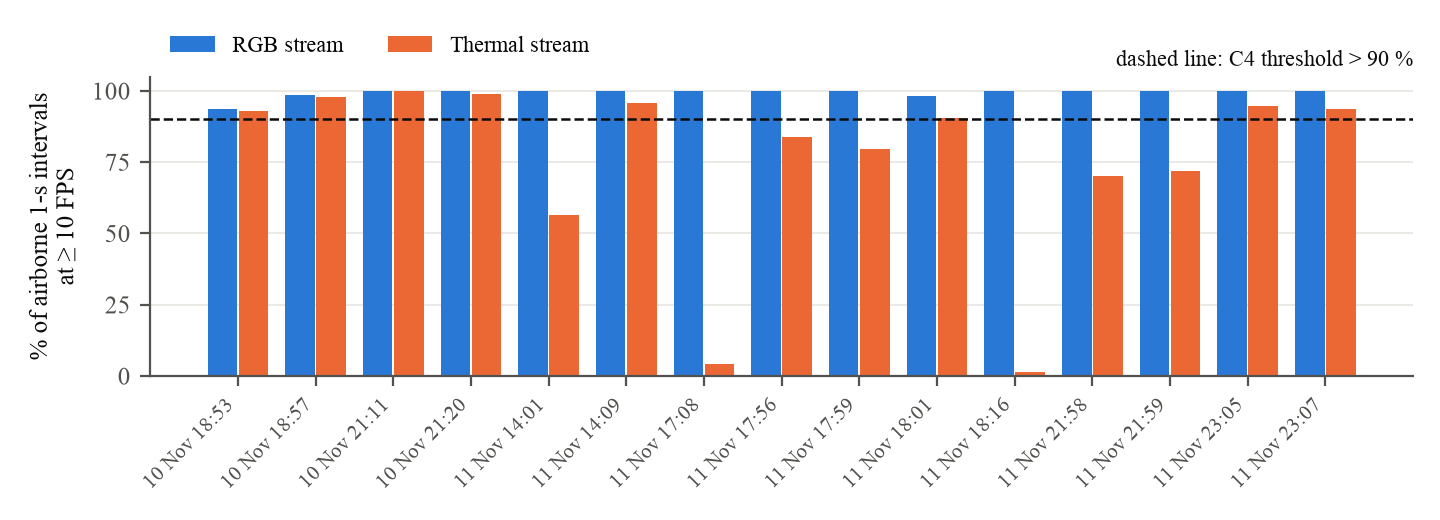
\includegraphics[width=\textwidth]{figures/chart_fps.png}
\caption{Share of airborne 1-s intervals at $\ge$ 10\,FPS per flight and stream (from \file{fps\_summary.json}).}
\end{figure}

\begin{figure}[!htb]
\centering
\begin{subfigure}{\textwidth}\centering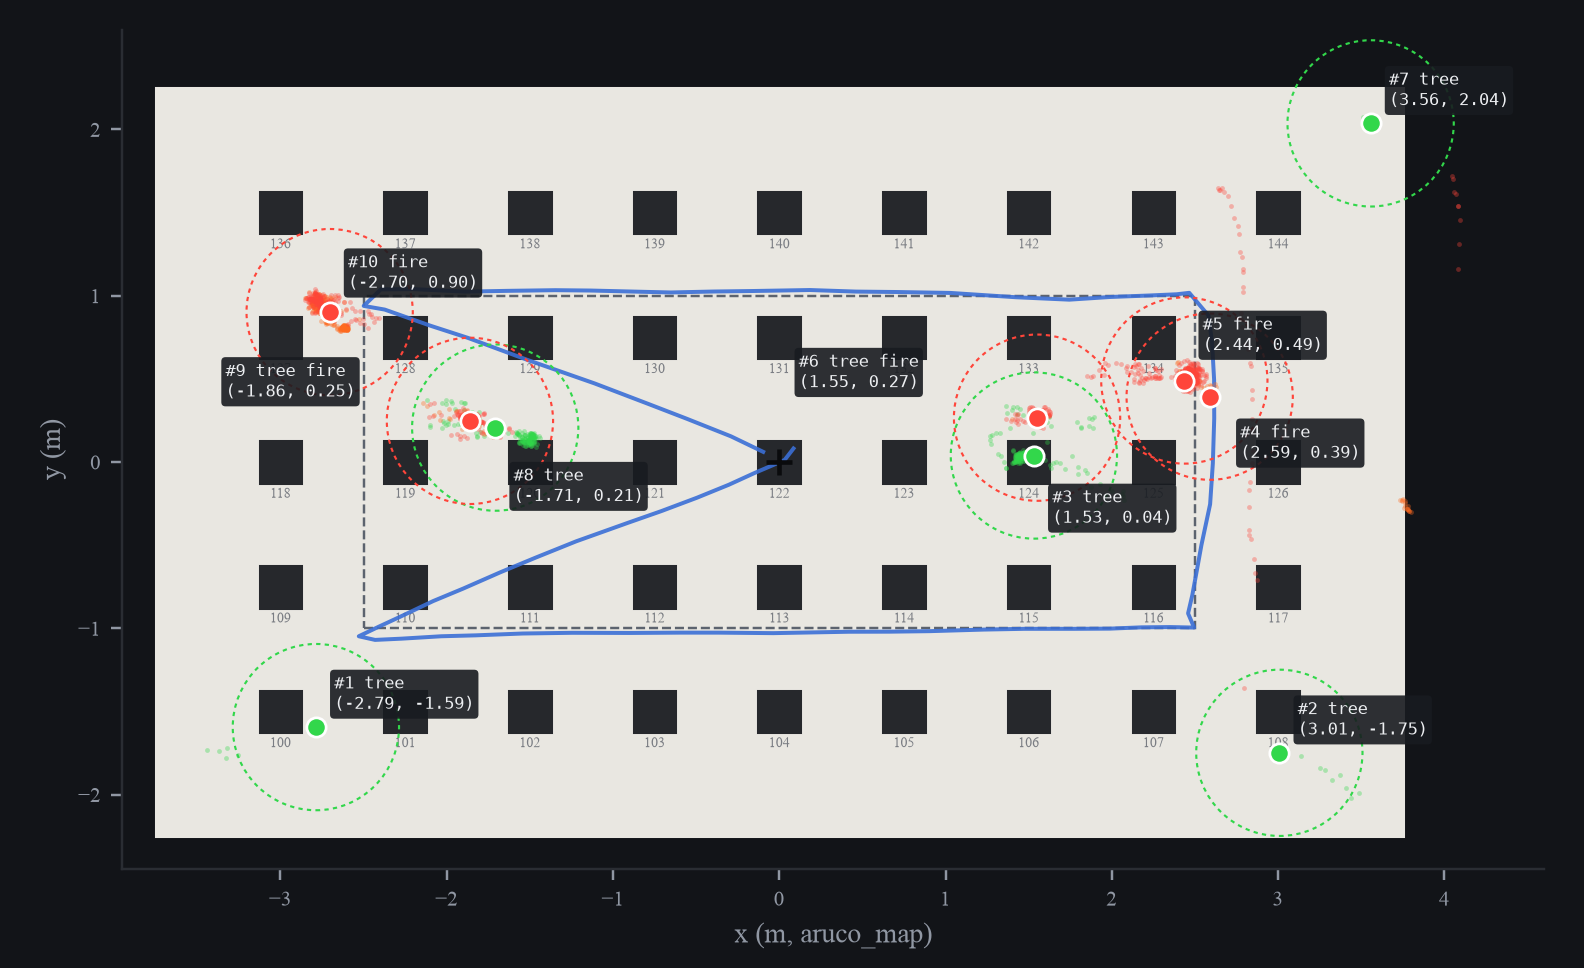
\includegraphics[width=0.74\linewidth]{figures/real_detmap.png}\caption{Detection map: all 1\,955 NN detections of the flight as dots (red = fire / tree heat band, orange = flame,
green = tree), the flown path (blue), the 10 confirmed objects with their reported X/Y and a 0.5\,m circle around each}\end{subfigure}\\[4pt]
\begin{subfigure}{\textwidth}\centering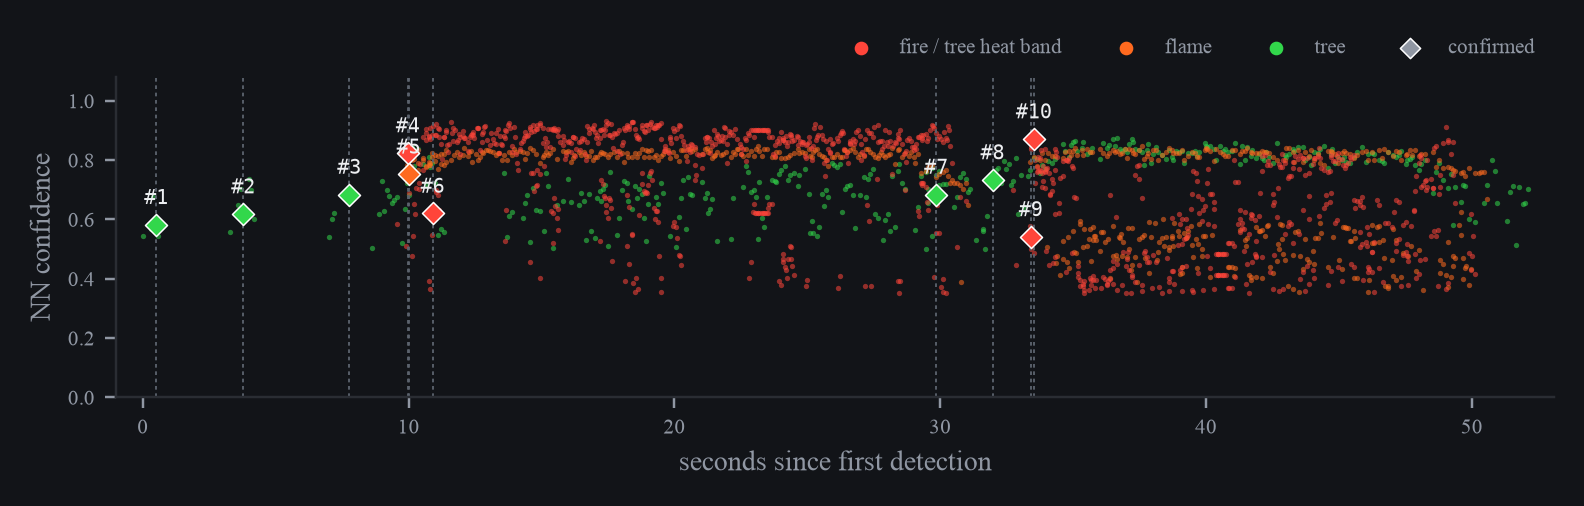
\includegraphics[width=\linewidth]{figures/real_events.png}\caption{Detection events: every dot is one detection (height = confidence); diamonds \#1--\#10 mark the moment each object was confirmed}\end{subfigure}
\caption{Real flight 11 Nov 23:07 (\file{case1\_fire\_20261111\_230709/events.csv}, \file{objects.json}, \file{path.csv}),
drawn in the dashboard's Results style. Most detections of each object fall inside its 0.5\,m circle.}
\label{fig:detmap}
\end{figure}

\subsection{C5 --- Object coordinate accuracy \hfill \PART}
Absolute accuracy is measured by the expert with a tape during the scored attempt, and the dashboard computes the error
per object (Judging Spec $\rightarrow$ C5). Two pieces of evidence were collected beforehand:
\begin{itemize}
  \item \textbf{Repeatability in flight.} The same objects were reported in four independent flights (11 Nov 21:58,
        21:59, 23:05, 23:07). Every report lies within 0.28\,m of the mean position for that object. Trees lie within
        0.10\,m and the campfires within 0.14--0.28\,m.
  \item \textbf{Absolute error in simulation.} With known ground truth, the campfire error is $\le$ 0.05\,m and the tree
        error is $\le$ 0.13\,m (Section~3.1).
\end{itemize}

\begin{figure}[!htb]
\centering
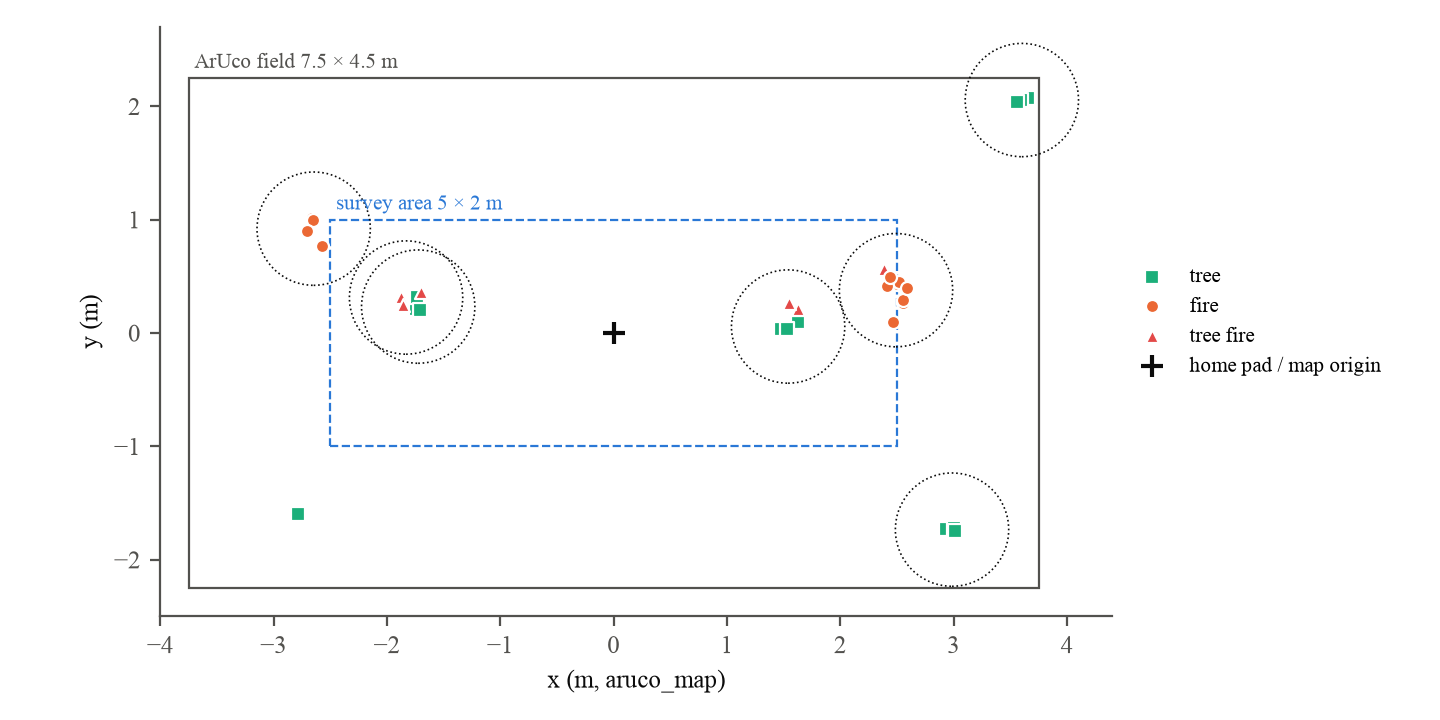
\includegraphics[width=0.72\textwidth]{figures/chart_repeat.png}
\caption{Object positions reported in four flights on the arena map. Dotted circles have a 0.5\,m radius around the mean
position of each object.}
\label{fig:repeat}
\end{figure}

\begin{tabularx}{\textwidth}{|L{2.4cm}|Y|L{2.1cm}|L{2.1cm}|L{3.6cm}|}
\hline
\rowcolor{headgray}\head{Object} & \head{Mean position (x, y)} & \head{Reports} & \head{Flights} & \head{Max deviation from mean} \\ \hline
Campfire A & (2.49, 0.38)\,m & 9 & 4 & 0.28\,m \\ \hline
Campfire B & ($-$2.65, 0.92)\,m & 4 & 4 & 0.17\,m \\ \hline
Heat band, tree 2 & ($-$1.83, 0.31)\,m & 4 & 4 & 0.14\,m \\ \hline
Tree 1 & (1.54, 0.06)\,m & 4 & 4 & 0.10\,m \\ \hline
Tree 2 & ($-$1.73, 0.23)\,m & 4 & 4 & 0.09\,m \\ \hline
Tree 3 & (2.99, $-$1.74)\,m & 4 & 4 & 0.06\,m \\ \hline
Tree 4 & (3.60, 2.06)\,m & 3 & 3 & 0.06\,m \\ \hline
\end{tabularx}


\begin{figure}[!htb]
\centering
\begin{subfigure}{0.49\textwidth}\centering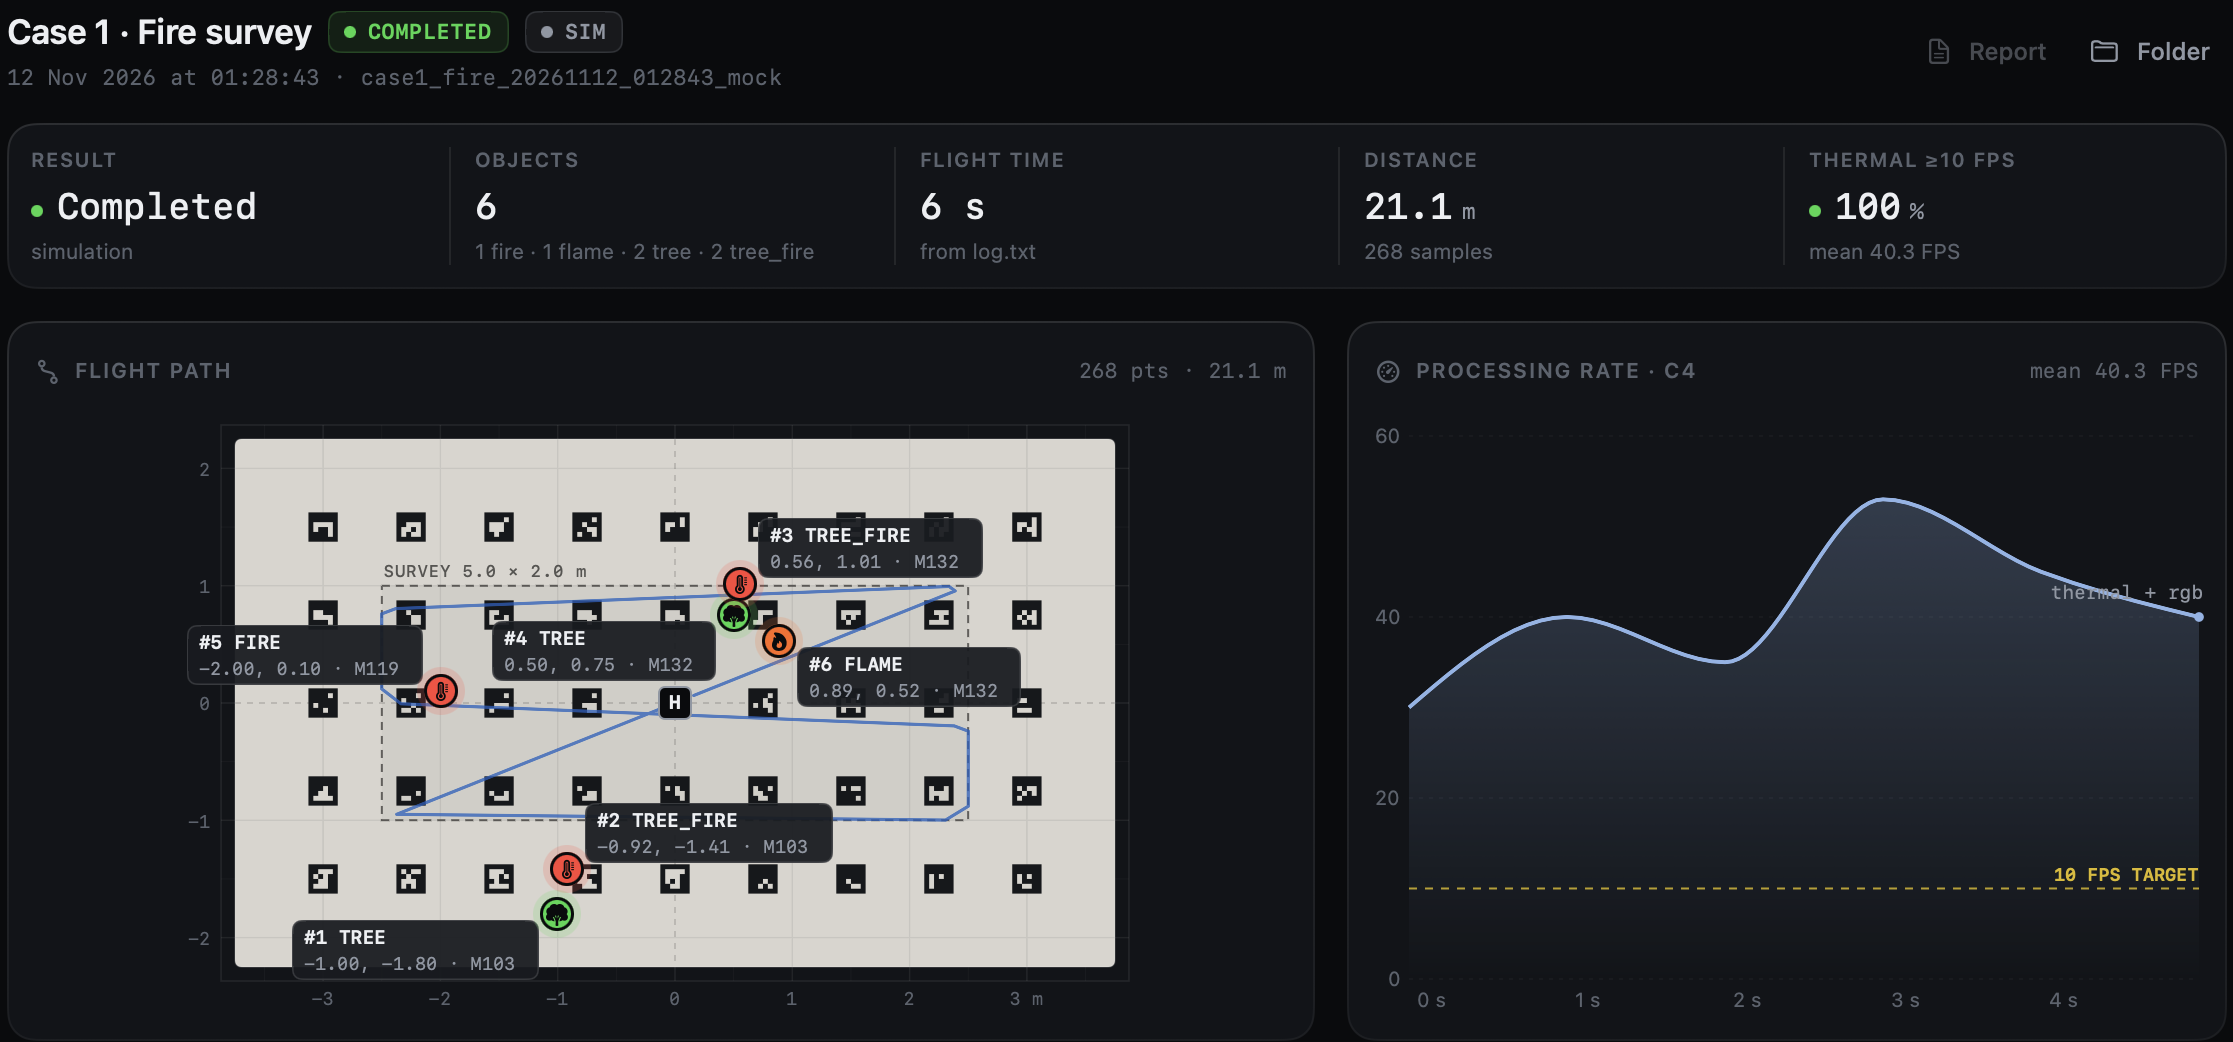
\includegraphics[width=\linewidth]{figures/ss_sim_path.png}\caption{Flight path with each confirmed object (class, X/Y, nearest marker) and processing rate}\end{subfigure}\hfill
\begin{subfigure}{0.49\textwidth}\centering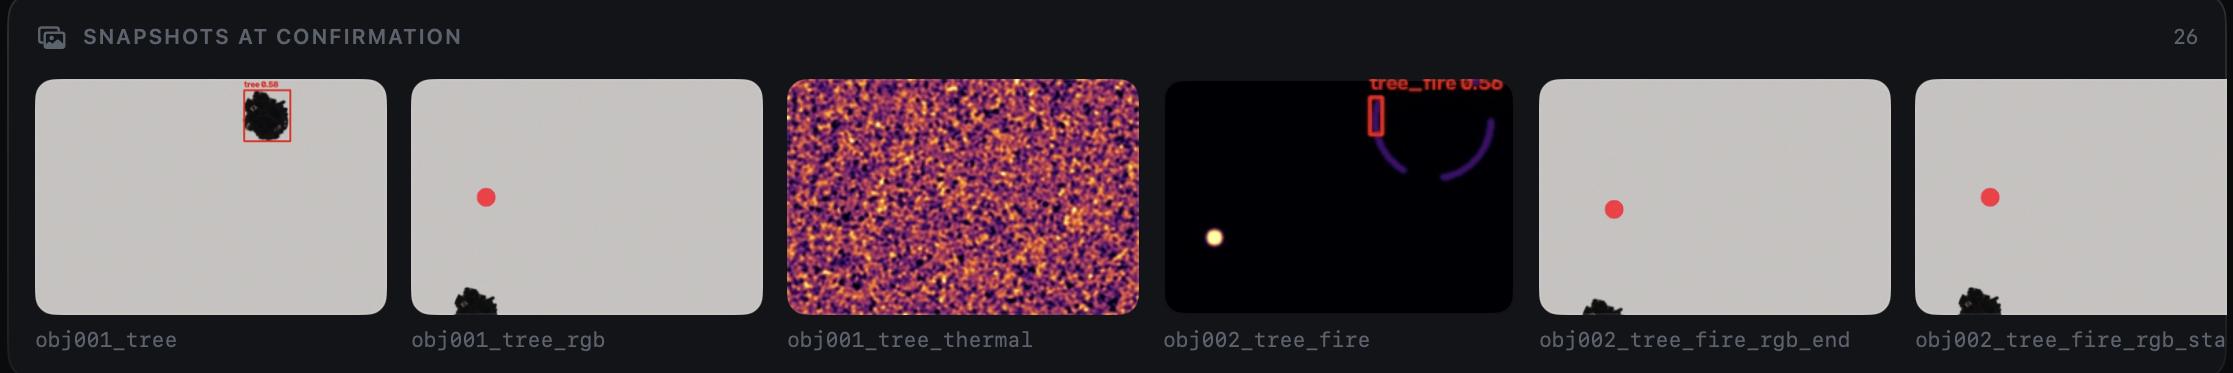
\includegraphics[width=\linewidth]{figures/ss_sim_snapshots.png}\caption{RGB and thermal snapshots taken at each confirmation}\end{subfigure}
\caption{Dashboard --- Results for a simulation run (12 Nov 01:28) with known target positions: the fire is reported at
($-$2.00, 0.10)\,m, exactly where it was placed.}
\end{figure}

\subsection{C6 --- Real-time display on the map \hfill \PART}
Each confirmed object appears on the live map in Mission Control and on the operator web UI with its class, X/Y and
confirmation time, and is added to the objects table. The dashboard polls the drone every 0.7\,s, and the link round
trip measured at the venue was 81--109\,ms. The expected display delay is therefore below 1\,s, against the 2\,s threshold.
The exact delay is measured from the screen recording of the scored attempt with the procedure in Section~2.2.



\subsection{C7 --- Autonomous return on operator command \hfill \PART}
\begin{itemize}
  \item \textbf{Return and landing in flight:} all 15 missions flew home autonomously and landed. The end of the return
        leg was 0.02--0.18\,m from the home pad (threshold 0.5\,m).
  \item \textbf{Operator command:} in the simulator, the RETURN press and the switch to the RETURN phase were logged in the
        same second (\texttt{06:38:35 operator pressed RETURN} $\rightarrow$ \texttt{06:38:35 [phase] RETURN}), so the
        reaction is under 1\,s against the 2\,s threshold. The command path (dashboard $\rightarrow$ HTTP $\rightarrow$
        mission) is the same in flight. The in-flight press is made at the scored attempt at a moment chosen by the expert.
\end{itemize}

\subsection{Event logging and detection in every flight}
Every detection is written to \file{events.csv} with timestamp, camera, class, confidence, X/Y/Z, object ID, drone pose and
temperature. Confirmed rows from the 11 Nov 23:07 flight:

\begin{table}[H]
\centering\small
\begin{tabular}{|l|l|l|c|c|c|c|}
\hline
\rowcolor{headgray}\head{Time} & \head{Camera} & \head{Class} & \head{Confidence} & \head{X (m)} & \head{Y (m)} & \head{Object} \\ \hline
23:07:30.658 & rgb & tree & 0.582 & $-$3.33 & $-$1.78 & 1 \\ \hline
23:07:37.921 & rgb & tree & 0.684 & 1.58 & 0.26 & 3 \\ \hline
23:07:40.124 & thermal & fire & 0.824 & 2.86 & $-$0.58 & 4 \\ \hline
23:07:40.155 & rgb & flame & 0.752 & 2.41 & 0.55 & 5 \\ \hline
23:07:41.058 & thermal & tree\_fire & 0.620 & 4.08 & 1.54 & 6 \\ \hline
23:08:02.122 & rgb & tree & 0.733 & $-$2.02 & 0.25 & 8 \\ \hline
23:08:03.678 & thermal & fire & 0.871 & $-$2.65 & 0.99 & 10 \\ \hline
\end{tabular}
\caption{Excerpt of \file{events.csv}: positions at the moment of confirmation. The tracker then refines each position
from all later views; the refined positions are reported in \file{objects.json} and on the map.}
\end{table}

A simulated flame (campfire or flame lamp) was confirmed in \textbf{15 of 15} complete missions, which meets the
``at least one detection per flight'' requirement.

% ------------------------------------------------------------------ 6
\section{Functional Modules and End-to-End Scenario}

\subsection{Module results}
\begin{tabularx}{\textwidth}{|L{3.0cm}|Y|L{1.9cm}|}
\hline
\rowcolor{headgray}\head{Module} & \head{Recorded result} & \head{Verdict} \\ \hline
M1 Flight and navigation & Hover tests on 9 and 10 Nov: hold at 1.42\,m and 1.37\,m (target 1.5 $\pm$ 0.15\,m), drift 0.08 / 0.03\,m, automatic landing and disarm (Section~4.1). & \PASS \\ \hline
M2 Thermal perception & In the 23:07 flight the thermal NN confirmed the campfire 0.08\,s after its first box (23:07:40.048 $\rightarrow$ 23:07:40.125), at confidence 0.82, with thermal processing at 16.6\,FPS. & \PASS \\ \hline
M3 Ground station and logging & Each confirmation appears on the map and in the table with type, X/Y and time (Figure~\ref{fig:results}); every detection is in \file{events.csv}; operator commands are logged with a timestamp. & \PASS \\ \hline
\end{tabularx}

\subsection{End-to-end scenario --- record of the 11 Nov 23:07 mission}
\begin{tabularx}{\textwidth}{|L{2.1cm}|Y|}
\hline
\rowcolor{headgray}\head{Time} & \head{Event (from \file{log.txt})} \\ \hline
23:07:09 & Settings loaded: area 5 $\times$ 2\,m, fence 6.6 $\times$ 3.5\,m, altitude 2.8\,m, speed 0.8\,m/s; battery 4.03\,V/cell \\ \hline
23:07:10--13 & Count-down (ABORT possible), pre-flight checks, take-off \\ \hline
23:07:22 & \texttt{aruco\_map} position acquired; survey starts (4 waypoints, 2 lines) \\ \hline
23:07:30--37 & Trees \#1--\#3 confirmed and mapped without stopping \\ \hline
23:07:41 & In-flight self-calibration: RGB views agree to 0.09\,m (were 0.17\,m), thermal to 0.03\,m (were 0.40\,m) \\ \hline
23:07:42--55 & Ignition sources \#4, \#5 (fire, 64--66\,$^\circ$C), \#6 (tree\_fire, 55\,$^\circ$C): LED alarm, 2\,s hold, snapshots \\ \hline
23:08:00--15 & Trees \#7, \#8 mapped; \#9 tree\_fire (49\,$^\circ$C), \#10 fire (69\,$^\circ$C): alarm, hold, snapshots \\ \hline
23:08:16 & Route complete $\rightarrow$ RETURN \\ \hline
23:08:21--32 & Landing, landed and disarmed \\ \hline
23:08:32 & Report written; mission result \texttt{completed} (78\,s, 17.5\,m, 10 objects) \\ \hline
\end{tabularx}

\textbf{Outcome:} intended result achieved: campfire detected, all objects mapped and logged, return and landing without
manual piloting, total time 1\,min 23\,s ($\le$ 9\,min). No non-critical failure occurred in this run.

\subsection{Additional functions}
\begin{tabularx}{\textwidth}{|L{0.8cm}|Y|L{1.9cm}|}
\hline
\rowcolor{headgray}\head{No.} & \head{Recorded result} & \head{Verdict} \\ \hline
AF1 & Every confirmed ignition source got an LED alarm, a 2\,s hold and start/end RGB + thermal snapshots (23:07 flight: 5 holds, 20 snapshot files). & \PASS \\ \hline
AF2 & Safety layer passes its unit tests (35/35). In flight the 4 navigation commands rejected outside OFFBOARD mode ended the attempt safely, and the fence and altitude limit from the configuration were applied in every mission. & \PASS \\ \hline
AF3 & Self-calibration ran in 11 of the 15 missions; on 23:07 it reduced the thermal view spread from 0.40\,m to 0.03\,m. & \PASS \\ \hline
\end{tabularx}

% ------------------------------------------------------------------ 7
\section{Defects Found and Corrective Actions}

\begin{longtable}{|L{0.6cm}|L{4.0cm}|L{4.1cm}|L{4.6cm}|L{1.7cm}|}
\hline
\rowcolor{headgray}\head{No.} & \head{Defect (evidence)} & \head{Root cause} & \head{Corrective action} & \head{Re-test} \\ \hline
\endfirsthead
\hline
\rowcolor{headgray}\head{No.} & \head{Defect (evidence)} & \head{Root cause} & \head{Corrective action} & \head{Re-test} \\ \hline
\endhead
D1 & A 100\,$^\circ$C thermal threshold rule never fired in flight & From flight height the campfire reads only 52--88\,$^\circ$C (sub-pixel averaging) & Fire detection is now NN-only; temperature only confirms NN boxes (fire $\ge$ 60, flame $\ge$ 50\,$^\circ$C) & Flight \PASS \\ \hline
D2 & Thermal 0.4\,FPS airborne (18:16), no frames at 17:25 while the RGB stream worked & TR256i re-enumerated on USB; the node only opened a fixed device path & Thermal node finds the camera on any USB port, 2\,s read timeout, reopens after 12\,s without a valid frame & Flight \PASS (23:05, 23:07) \\ \hline
D3 & Thermal node CPU load: a false-colour image was built 25$\times$/s and discarded & Unneeded processing in the camera node & Decode only the temperature data; colourise only when a picture is shown & Self-test \PASS, flight pending \\ \hline
D4 & Tree positions 3$\times$ worse after self-calibration (lens $\times$0.65) & Unbounded lens scale & Lens scale limited to 0.75--1.33 & Unit test + flight \PASS \\ \hline
D5 & Trees at the picture edge never mapped (107/117 views) & Tracker opened objects only from central views & Edge classes (\texttt{tree}, \texttt{tree\_fire}) accepted at the edge & Flight \PASS \\ \hline
D6 & Old thermal model labelled tree heat bands as \texttt{flame} & No heat-band class in training data & New thermal model v3 with class \texttt{tree\_fire} (hand-checked frames) & Flight \PASS \\ \hline
D7 & Dashboard link 479\,ms average, 1.3\,s maximum with video & 3.7\,Mbit/s of full-rate video on the venue Wi-Fi & ``Data saver'' video mode (480 $\times$ 360, 93\,KB/s); status timeout 4\,s, link lost only after 8\,s & Measured \PASS \\ \hline
D8 & 3 of 5 screen recordings unplayable (no moov atom) & Equal timestamps on two frames stopped the encoder & Microsecond timestamps, 2\,s fragments, continue in a new part file on error & Bench \PASS \\ \hline
D9 & Three back-to-back holds took 13\,s; each LED flash blocked 1--2\,s & One hold per source; blocking LED call & One shared hold for sources confirmed together; non-blocking LED queue & Unit test \PASS, flight pending \\ \hline
D10 & 3\,m altitude refused by the drone & Deployed limit 3.0\,m, ceiling 3.5\,m & Limit 3.2\,m (instant landing at 3.45\,m), cruise 2.9\,m & Unit test \PASS, flight pending \\ \hline
\end{longtable}

Defects D1, D2 and D4--D8 were corrected and re-tested before the final flights on 11 November. D3, D9 and D10 were
corrected on 12 November and verified by self-tests and unit tests. Their in-flight verification is scheduled for the next flight-area slot. No
thresholds or test conditions were changed as a result of the defects.

% ------------------------------------------------------------------ 8
\section{Photographic and Video Evidence}

\begin{figure}[!htb]
\centering
\begin{subfigure}{0.48\textwidth}\centering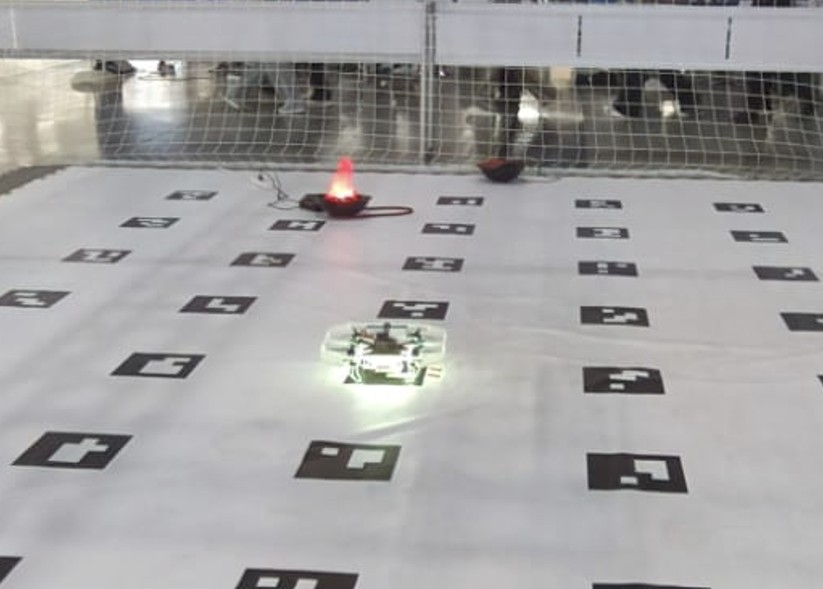
\includegraphics[width=\linewidth,height=3.3cm,keepaspectratio]{figures/photo_hover.png}\caption{Hover test, 9 Nov}\end{subfigure}\hfill
\begin{subfigure}{0.48\textwidth}\centering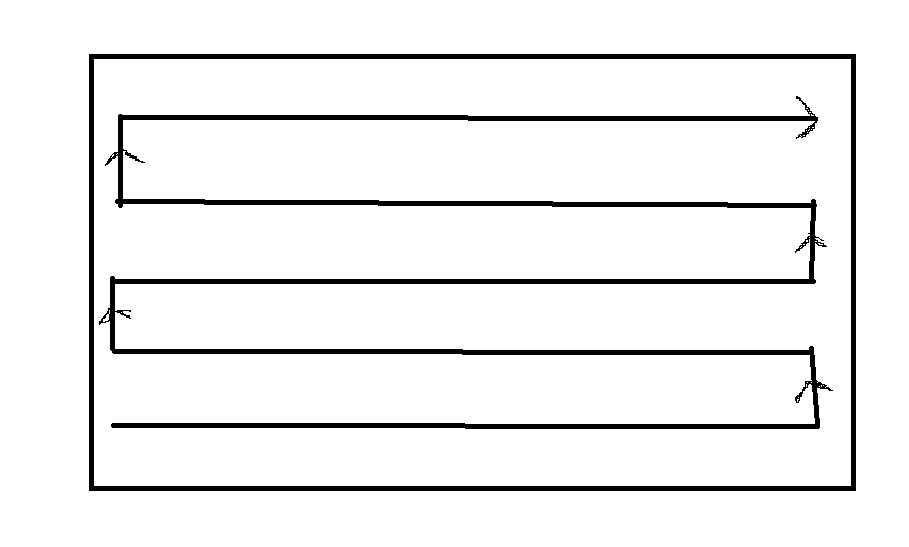
\includegraphics[width=\linewidth,height=3.3cm,keepaspectratio]{figures/photo_survey.png}\caption{Autonomous survey route}\end{subfigure}\\[4pt]
\begin{subfigure}{0.48\textwidth}\centering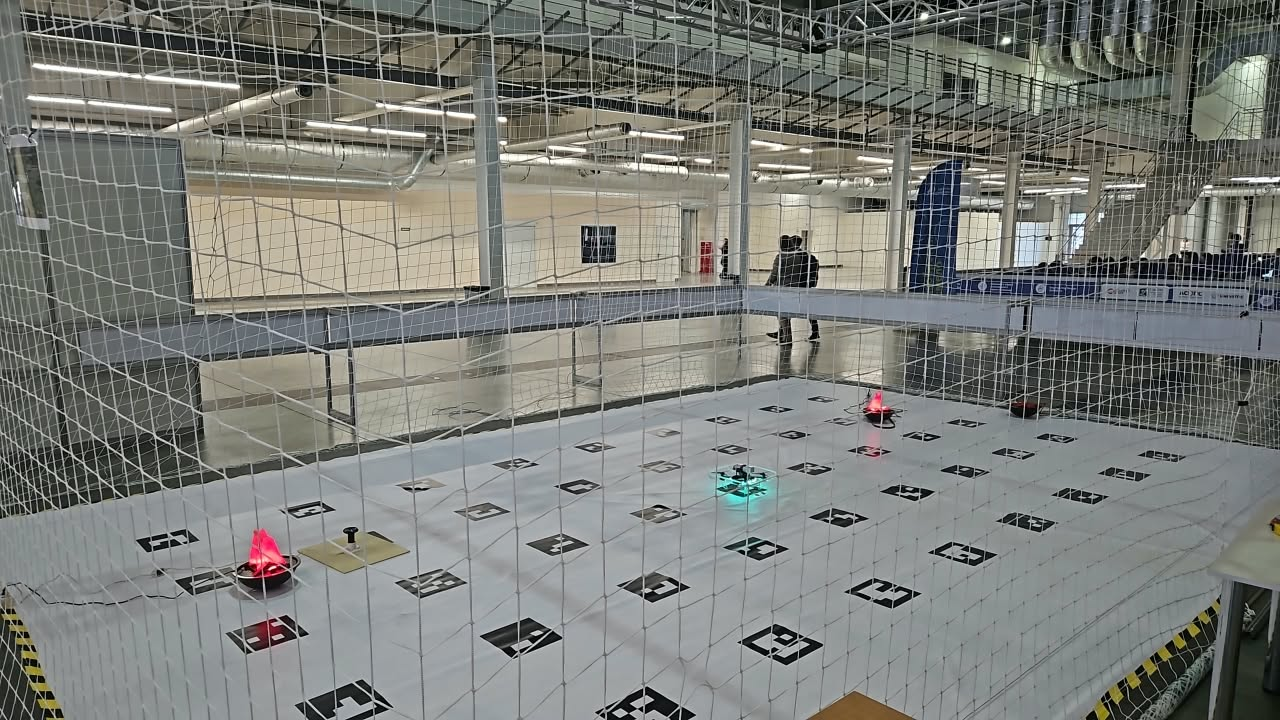
\includegraphics[width=\linewidth,height=3.3cm,keepaspectratio]{figures/photo_area.png}\caption{Aircraft in the test area}\end{subfigure}\hfill
\begin{subfigure}{0.48\textwidth}\centering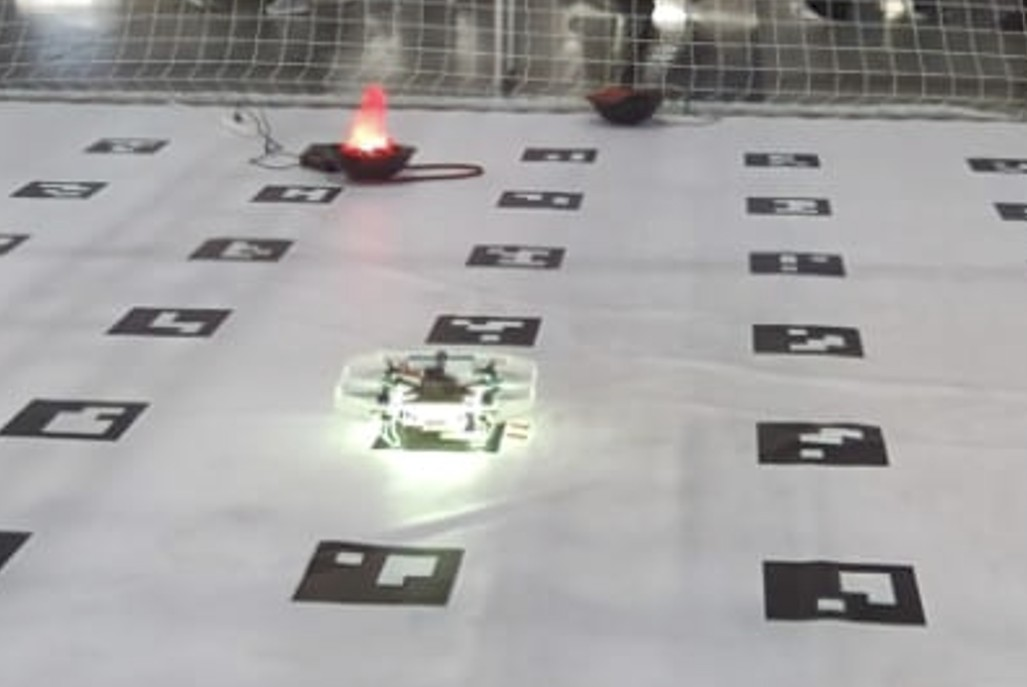
\includegraphics[width=\linewidth,height=3.3cm,keepaspectratio]{figures/photo_landing.png}\caption{Autonomous landing}\end{subfigure}
\caption{Flight-test photographs, competition flight area, 9--10 November 2026.}
\end{figure}

\begin{figure}[!htb]
\centering
\begin{subfigure}{0.24\textwidth}\centering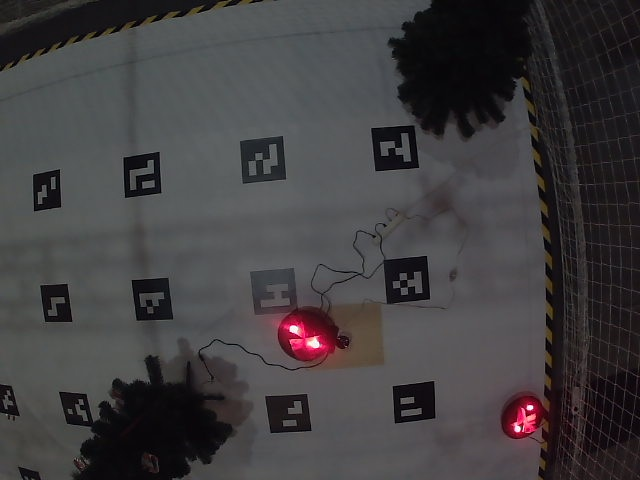
\includegraphics[width=\linewidth]{figures/ev_obj005_fire_rgb_start.jpg}\caption{\#5 campfire, RGB}\end{subfigure}\hfill
\begin{subfigure}{0.24\textwidth}\centering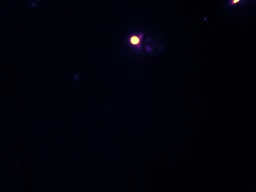
\includegraphics[width=\linewidth]{figures/ev_obj005_fire_thermal_start.jpg}\caption{\#5 campfire, thermal}\end{subfigure}\hfill
\begin{subfigure}{0.24\textwidth}\centering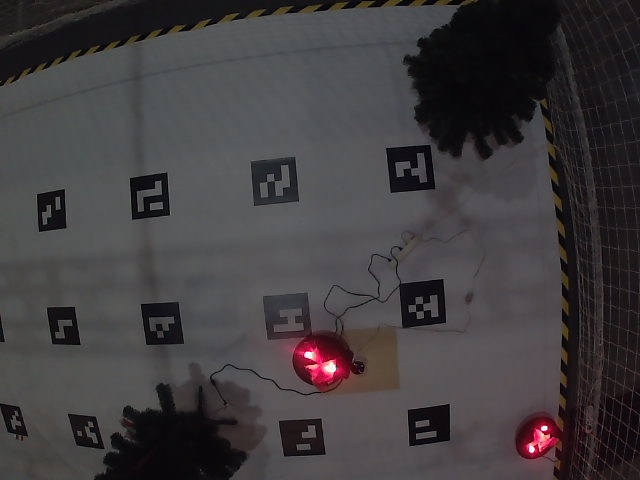
\includegraphics[width=\linewidth]{figures/ev_obj003_tree_rgb.jpg}\caption{\#3 tree, RGB}\end{subfigure}\hfill
\begin{subfigure}{0.24\textwidth}\centering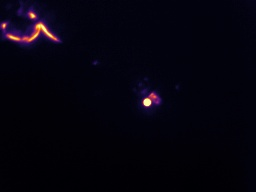
\includegraphics[width=\linewidth]{figures/ev_obj009_tree_fire_thermal_start.jpg}\caption{\#9 heat band, thermal}\end{subfigure}
\caption{Snapshots taken automatically by the drone during the inspection hold (11 Nov 23:07 flight,
\file{snapshots/obj00x\_*.jpg}).}
\end{figure}

\begin{figure}[!htb]
\centering
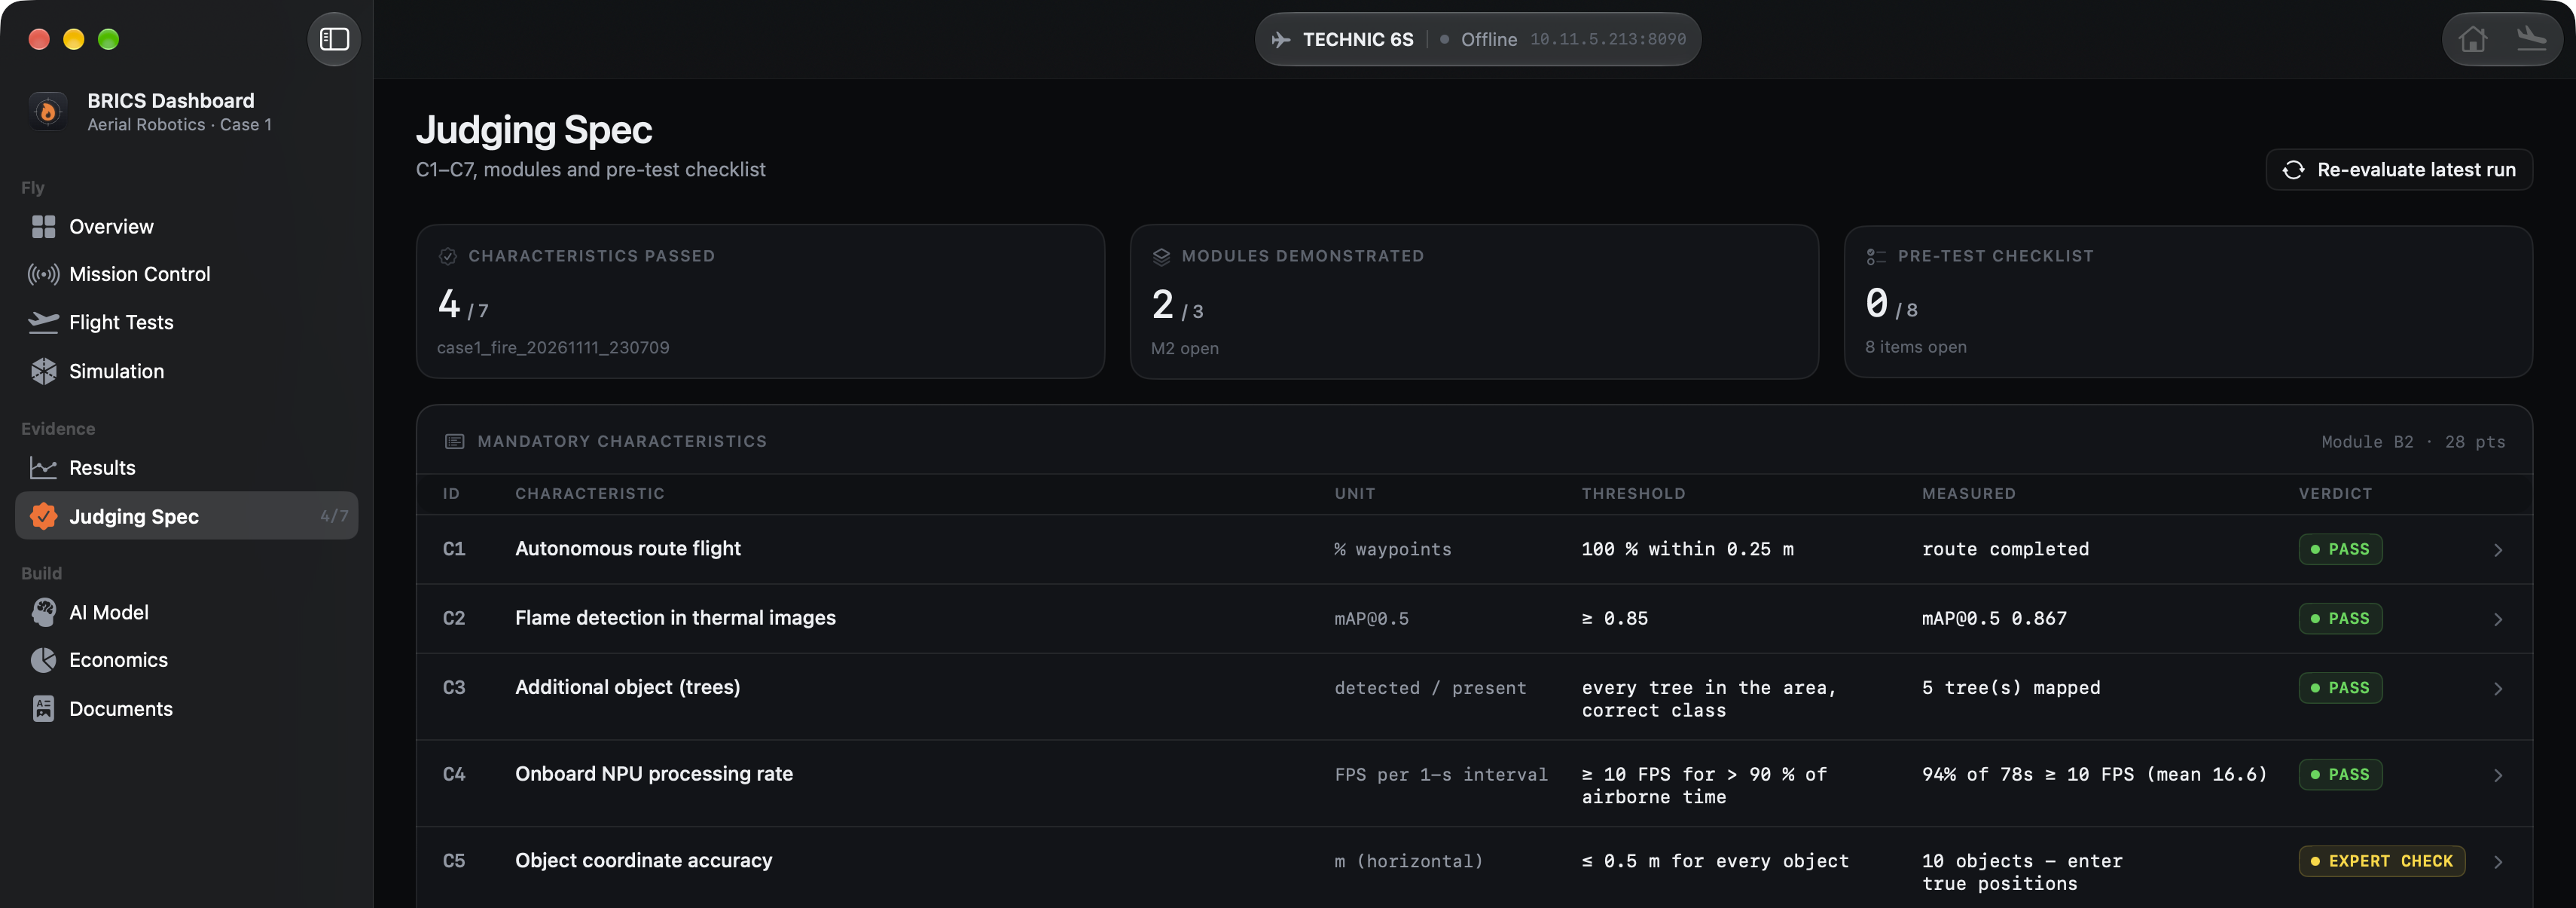
\includegraphics[width=\textwidth]{figures/dash_spec.png}
\caption{Dashboard --- Judging Spec: C1--C7 scored automatically from the latest flight run folder
(\file{case1\_fire\_20261111\_230709}); C5 waits for the expert's tape measurements.}
\end{figure}


\textbf{Video:} every attempt is screen-recorded by the dashboard (REC, MP4 per camera) and the flight area is filmed
continuously. Recordings and all run folders are stored in \file{BRICS Mission Logs/} and are available to the experts.

% ------------------------------------------------------------------ 9
\section{Requirement Traceability and Conclusions}

\subsection{Case 1 requirements}
\begin{tabularx}{\textwidth}{|L{0.6cm}|Y|L{1.3cm}|L{4.3cm}|L{1.7cm}|}
\hline
\rowcolor{headgray}\head{No.} & \head{Case 1 requirement} & \head{Test} & \head{Evidence} & \head{Status} \\ \hline
1 & Autonomous flight along a predefined route & C1, M1 & Table~\ref{tab:flights}, route chart & \PASS \\ \hline
2 & Onboard thermal camera, real-time thermograms & M2, C4 & thermal FPS, snapshots & \PASS \\ \hline
3 & NN flame detection in thermal images, mAP@0.5 $\ge$ 85\,\% & C2 & validation table, PR curve & \PASS \\ \hline
4 & At least one additional object & C3 & trees in 4/4 flights & \PASS \\ \hline
5 & NPU/GPU processing $\ge$ 10\,FPS for $>$ 90\,\% of time & C4 & FPS chart & \PASS \\ \hline
6 & Coordinates $\le$ 0.5\,m, sent to the interface & C5 & repeatability, simulation & \PART \\ \hline
7 & Real-time map with type and timestamp & C6, M3 & dashboard screenshots & \PART \\ \hline
8 & Logging of time, coordinates, type, confidence & M3 & \file{events.csv} excerpt & \PASS \\ \hline
9 & At least one flame detection per flight & E2E & 15/15 missions & \PASS \\ \hline
10 & Autonomous return on operator command & C7 & return error chart, simulation log & \PART \\ \hline
\end{tabularx}

\subsection{Evidence index for the experts}
Each test record (TR) points to the files that prove it. Run folders are in \file{BRICS Mission Logs/} and in the project
repository (\url{https://github.com/kkjjkamal123/BRICS-HiTech-2026-Flying-Robotics}).

\begin{tabularx}{\textwidth}{|L{1.1cm}|L{3.3cm}|Y|L{2.6cm}|}
\hline
\rowcolor{headgray}\head{TR} & \head{Test} & \head{Evidence files} & \head{Report section} \\ \hline
TR-01 & C1 route & 15 run folders: \file{log.txt} \texttt{[plan]}, \file{path.csv}; \file{make\_figures.py} & 5.1, Table~\ref{tab:flights} \\ \hline
TR-02 & C2 thermal mAP & \file{models/thermal\_fire/best.pt}, \file{datasets/thermal\_fire\_v3} (val), Ultralytics \texttt{val} & 3.2, 5.2 \\ \hline
TR-03 & C3 trees & \file{case1\_fire\_20261111\_215809 / 215959 / 230513 / 230709}: \file{objects.json}, \file{snapshots/} & 5.3 \\ \hline
TR-04 & C4 FPS & every run: \file{perf.csv}, \file{fps\_summary.json} & 5.4 \\ \hline
TR-05 & C5 coordinates & 4 evening runs: \file{objects.json}; \file{tests/sim\_case1\_venue.py} & 5.5 \\ \hline
TR-06 & C6 live map & dashboard Results / Mission Control; screen recording of the scored attempt & 5.6 \\ \hline
TR-07 & C7 return & all runs: \file{log.txt} \texttt{[phase] RETURN}, \file{path.csv}; simulator log & 5.7 \\ \hline
TR-08 & M1--M3, end-to-end & \file{flight\_logs/hover\_*.csv}; \file{case1\_fire\_20261111\_230709/log.txt}, \file{events.csv} & 6 \\ \hline
TR-09 & Software tests & \file{tests/test\_flight\_safety.py}, \file{tests/run\_all\_tests.py --quick} & 3.1 \\ \hline
\end{tabularx}

\subsection{Conclusions}
\begin{itemize}
  \item The prototype flew 15 complete autonomous missions without manual piloting. It reached every planned waypoint
        within 0.09\,m and returned within 0.18\,m of home.
  \item The thermal NN exceeds the mAP@0.5 threshold on held-out flight frames (0.993 for the campfire), and the campfire
        was detected in every mission.
  \item Testing exposed a thermal-camera stream fault that failed C4 in seven flights. It was traced to the USB camera
        driver path and corrected; both streams then met C4 in the final flights.
  \item Coordinate accuracy, display delay and the in-flight operator RETURN are supported by the recorded evidence. Their
        final values are measured during the scored attempt with the pre-agreed procedures.
\end{itemize}

\begin{center}\textbf{END OF TEST REPORT} --- Module B: Prototype Functional Verification\end{center}

\end{document}
